\section{Mengenal Python}
Python adalah bahasa pemrograman interpretatif multiguna. Tidak seperti bahasa lain yang susah untuk dibaca dan dipahami, python lebih menekankan pada keterbacaan kode agar lebih mudah untuk memahami sintaks. Hal ini membuat Python sangat mudah dipelajari baik untuk pemula maupun untuk yang sudah menguasai bahasa pemrograman lain. Bahasa ini muncul pertama kali pada tahun 1991, dirancang oleh seorang bernama Guido van Rossum. Sampai saat ini Python masih dikembangkan oleh Python Software Foundation. Bahasa Python mendukung hampir semua sistem operasi, bahkan untuk sistem operasi Linux, hampir semua distronya sudah menyertakan Python di dalamnya. Dengan kode yang simpel dan mudah diimplementasikan, seorang programmer dapat lebih mengutamakan pengembangan aplikasi yang dibuat, bukan malah sibuk mencari syntax error.

Contoh syntax python sederhana:
\begin{lstlisting}[language=Python]
print("aku suka python")
\end{lstlisting}

Hanya dengan menuliskan kode print seperti yang diatas, anda sudah bisa mencetak apapun yang anda inginkan di dalam tanda kurung \textbf{()}. Dibagian akhir kode pun, anda tidak harus mengakhirnya dengan tanda semicolon \textbf{;}.

\section{Kelebihan Python}
Berdasarkan survey yang dilakukan oleh situs stackoverlow, Bahasa pemrograman python merupakan bahasa yang menduduki urutan pertama sebagai bahasa yang paling banyak dibahas di dunia. Karena memiliki kelebihan atau keunggulan yang membuat bahasa satu ini digemari banyak orang diseluruh dunia. Keunggulan tersebut antara lain ;
\begin{enumerate}
\item Memiliki library yang luas dan banyak; Bahasa pemrograman python memiliki banyak library yang siap anda gunakan yang berisi berbagai modul. Didalamnya terdapat berbagai macam kode untuk digunakan seperti regulas expressions, documentation-generation, unit testing, database, CGI, email, dan masih banyak lagi. Sehingga dengan adanya library ini, anda tidak perlu menulis lagi secara manual
\item Open Source atau gratis; Python merupakan bahasa pemrograman open source atau dapat anda unduh secara gratis. Bahasa satu ini dikembangkan dibawah lisensi open source yang disetujui oleh OSI dimana bahasa pemrograman ini bebas digunakan, dikembangkan, dan di distribusikan, bahkan termasuk tujuan komersial.
\item Mampu meningkatkan produktifitas developer; Sebagai bahasa yang mudah digunakan dan dipelajari membuat developer menjadi lebih produktif, apa lagi disertai dengan library yang luas. Selain itu dengan bahasa python, anda hanya perlu menulis kode lebih sedikit sehingga anda mempunyai banyak waktu untuk bisa mengerjakan yang lain.
\item Mendukung Internet Of Things (IoT) yang baik; Manfaat yang bisa anda dapatkan ketika menggunakan bahasa pemrograman python salah satunya yaitu mampu mendukung ekosistem Internet Of Things (IoT) dengan sangat baik, dimana python mampu menghubungkan benda-benda disekitar lingkungan kita kedalam sebuah internet yang menghubungkan satu sama lain.
\item Bahasa yang mudah dipelajari dan mudah digunakan; Python merupakan bahasa yang mudah dipelajari bahkan untuk pengembang pemula. Kode bahasa python ini mudah dibaca dan bisa menjalankan banyak fungsi kompleks dengan mudah, karena banyaknya library. Selain itu, proses pengembangan bahasa python bisa dilakukan dengan cepat menggunakan kode yang lebih sedikit. Bahkan tim kecil pun bisa menangani bahasa python secara efektif. Python merupakan bahasa yang sangat dinamis dimana dibangun berdasarkan tingkat keterbacaan kode yang tinggi. Sehingga kode tersebut mudah dipahami dan dicerna. Berbagai macam jenis library memuat banyak perlengkapan dan fungsionalitas yang sangat luar biasa, sehingga kemudahan dalam membangun program menjadi salah satu yang ditawarkan oleh bahasa pemrograman satu ini.
\item Fleksibel; Kode program yang ditulis menggunakan bahasa python dapat dijalankan di hampir semua sistem operasi seperti Windows, Mac, maupun Linux, termasuk beberapa perangkat-perangkat seluler. Kode python dapat di integrasikan dengan aplikasi yang ditulis dalam bahasa pemrograman lain dengan mekanisme tertentu. Misal, kode python dapat dipanggil dari kode C/C++, dan sama halnya dengan perkembangan .NET Framework.
\end{enumerate}

\section{Kekurangan Python}
Selain kelebihan diatas, bahasa pemrograman python juga memiliki kekurangan. Seperti halnya bahasa yang lain, tidak ada bahasa pemrograman yang sempurna. Berikut ulasan lengkap mengenai apa saja kelemahan bahasa pemrograman python.
\begin{enumerate}
\item Tidak cocok untuk aplikasi mobile; Python merupakan bahasa pemrograman yang sangat baik digunakan untuk platform dekstop dan server namun tidak dalam urusan komputasi aplikasi mobile. Pengembangan aplikasi dan game kurang cocok jika menggunakan python. Bahkan banyak yang mengatakan bahwa mustahil membuat game dalam bentuk tiga dimensi dengan grafis tinggi menggunakan python.
\item Eksekusi relatif lambat; Python merupakan bahasa interpreter yang bekerja dengan menggunakan kompiler. Dimana ketika dijalankan, python akan bekerja lebih lambat jika dibandingkan dengan bahasa lain. Tetapi hal ini juga bergantung dari besar dan kecilnya program yang akan kita buat. Python tidak baik jika diperuntukkan dalam pekerjaan multi-processor atau multi-core. Python dinilai memiliki performa yang relatif lambat jika dibandingkan dengan bahasa pemrograman lainnya. Bahkan beberapa penugasan terdapat diluar dari jangkauan python, serupa bahasa pemrograman dinamis lainnya, python tidak secepat atau efisien sebagai statis, tidak seperti bahasa pemrograman compilasi serupa bahasa C.
\item Kesulitan jika beralih ke bahasa pemrograman lain; Python memiliki banyak library yang luas sehingga pengguna python terbiasa dengan fitur yang ada pada library tersebut. Hal ini tentu saja dapat menimbulkan masalah seperti pengguna mengalami kesulitan ketika belajar maupun beralih ke bahasa pemrograman yang lain. Karena kebiasaan menggunakan library tersebut membuat pengguna tidak mengetahui bagaimana asal pembuatan source code library tersebut.
\item Kesalahan saat runtime; Python merupakan bahasa pemrograman yang dinamis, dimana anda tidak perlu mendeklarasikan tipe variabel saat menulis kode. Meskipun ini memudahkan developer selama pengkodean, namun pastinya dapat meningkatkan terjadinya kesalahan saat run-time.
\item Efisiensi dan fleksibilitas tradeoff by; Python memberikan flesibilitas tradeoff by dengan tidak diberikan secara meluas. Python menyiapkan bahasa pemrograman optimasi untuk kegunaan bersama dengan perangkat bantu yang dibutuhkan untuk di integrasikan dengan bahasa pemrograman lain.
\end{enumerate}


\section{Instalasi Python}
Sebelum Anda menggunakan Python, Anda harus menginstalnya terlebih dahulu di sistem operasi komputer Anda. Saat ini Python memiliki 2 versi yang berbeda, yaitu Python versi 3 dan Python versi 2. Disini kita akan belajar bahasa pemrograman Python menggunakan versi terbaru 3. Cara menginstal python sangat mudah, ikuti panduan dibawah ini. Dibawah adalah panduan cara instal python di platform Linux, dan Windows

\subsection{Linux}
\subsubsection{Anaconda}
\begin{enumerate}
\item Buka browser, kunjungi \url{https://www.anaconda.com/products/individual}.
\item lalu scroll sampai muncul menu seperti gambar dibawah, klik kanan pada Installer dan klik \textbf{Copy link address}
\begin{figure}[H]
        \centerline{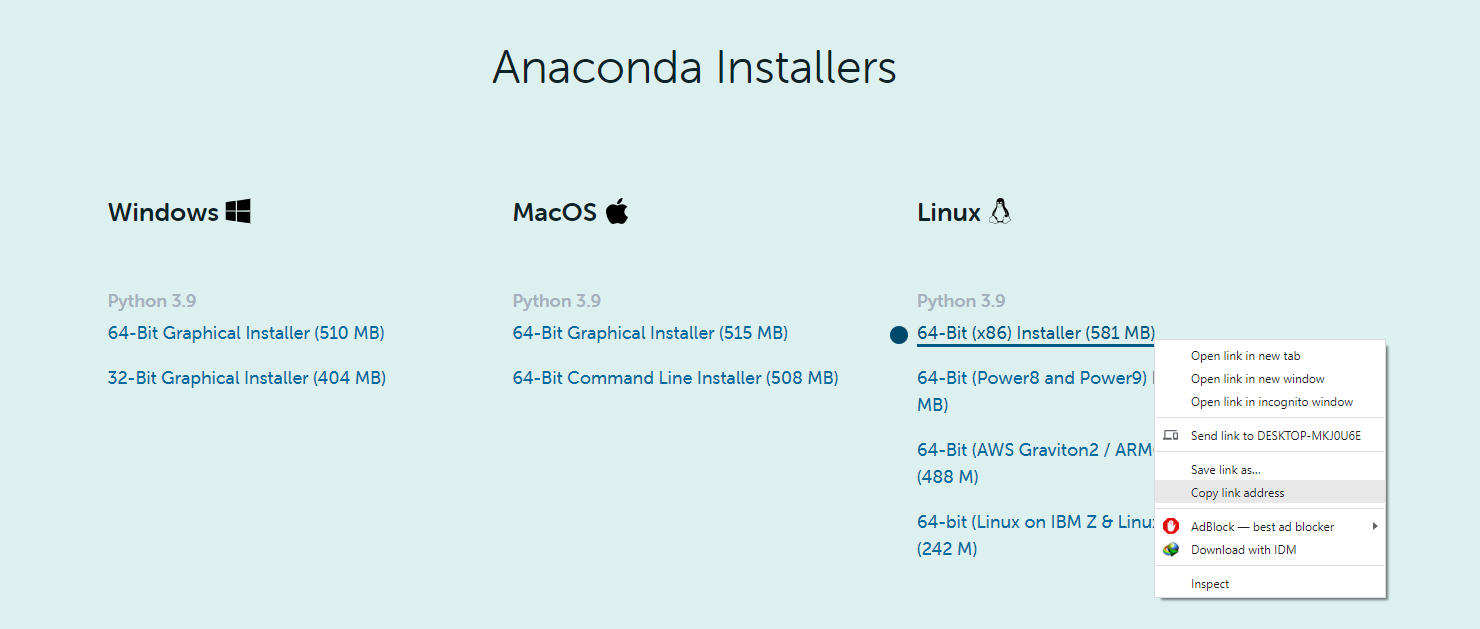
\includegraphics[scale=0.35]{figures/instalasi-anaconda-linux/step1}}
        \caption{Instalasi Anaconda Linux: Step 1}
\end{figure}
\item buka terminal lalu ketikkan \textbf{cd temp/}, tekan enter
\begin{figure}[H]
        \centerline{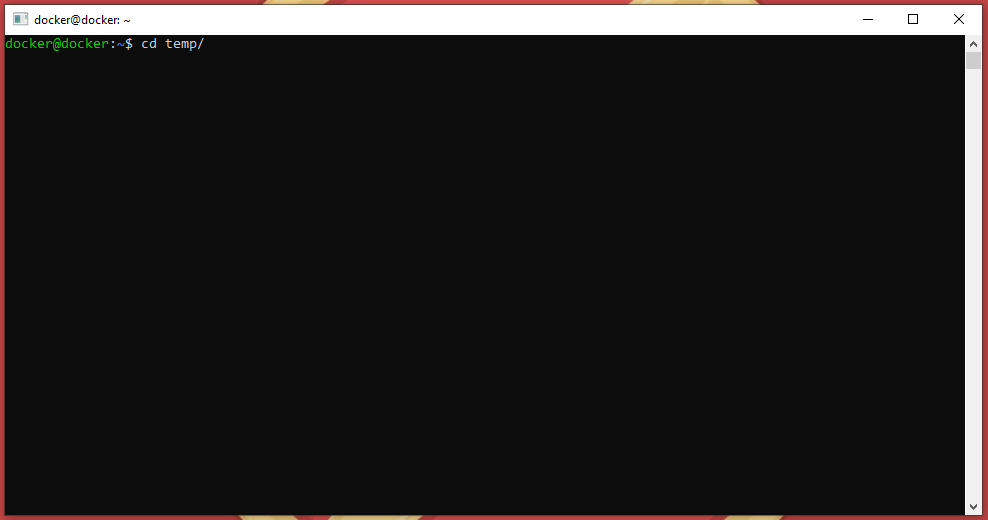
\includegraphics[scale=0.5]{figures/instalasi-anaconda-linux/step2}}
        \caption{Instalasi Anaconda Linux: Step 2}
\end{figure}
\item setelah itu ketikkan \textbf{wget \textit{link yang sudah dicopy}}
\begin{figure}[H]
        \centerline{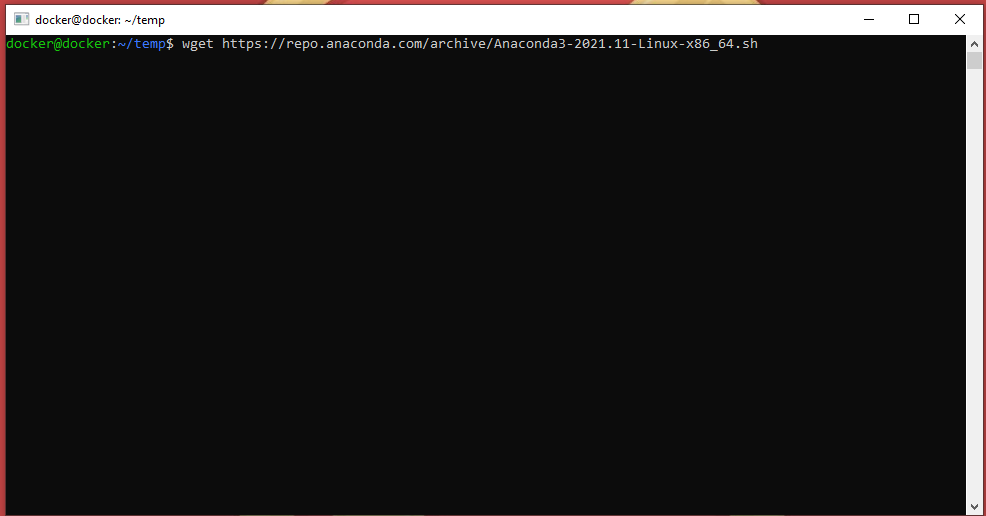
\includegraphics[scale=0.5]{figures/instalasi-anaconda-linux/step3}}
        \caption{Instalasi Anaconda Linux: Step 3}
\end{figure}
\item tekan enter, dan tunggu hingga download selesai
\begin{figure}[H]
        \centerline{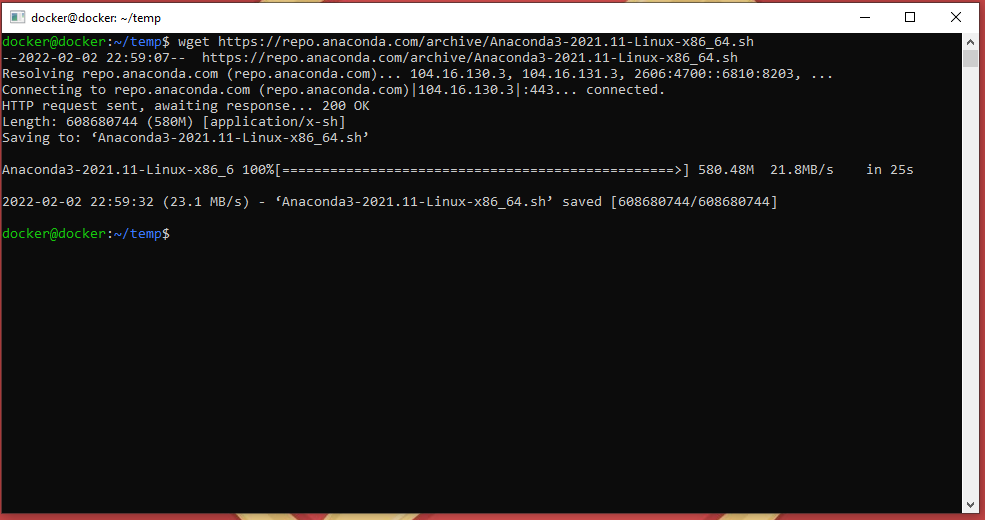
\includegraphics[scale=0.5]{figures/instalasi-anaconda-linux/step4}}
        \caption{Instalasi Anaconda Linux: Step 4}
\end{figure}
\item jika sudah ketikkan \textbf{bash \textit{nama file anaconda, sedikit tips, untuk lebih cepat ketikkan Anac lalu tekan Tab maka secara otomatis akan mengisi nama filenya}}
\begin{figure}[H]
        \centerline{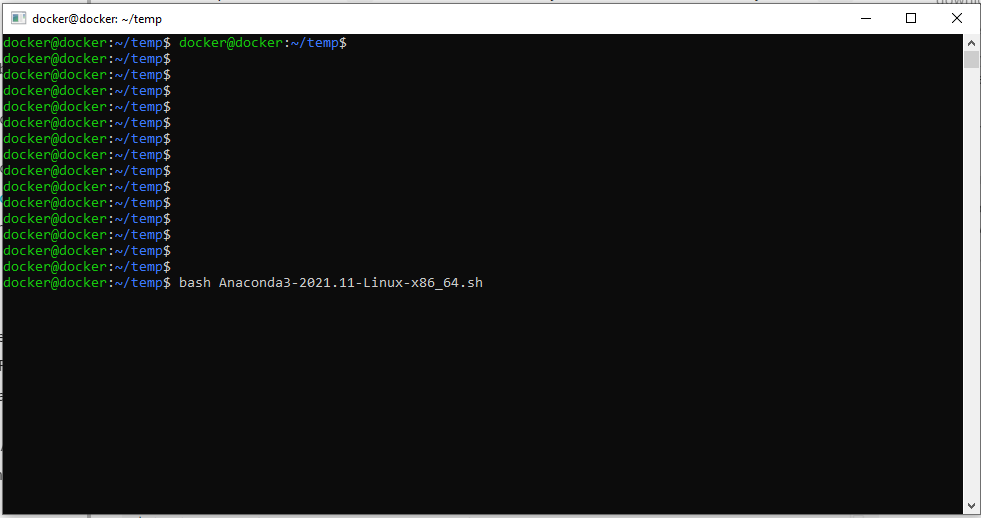
\includegraphics[scale=0.5]{figures/instalasi-anaconda-linux/step5}}
        \caption{Instalasi Anaconda Linux: Step 5}
\end{figure}
\item lalu tekan Enter
\begin{figure}[H]
        \centerline{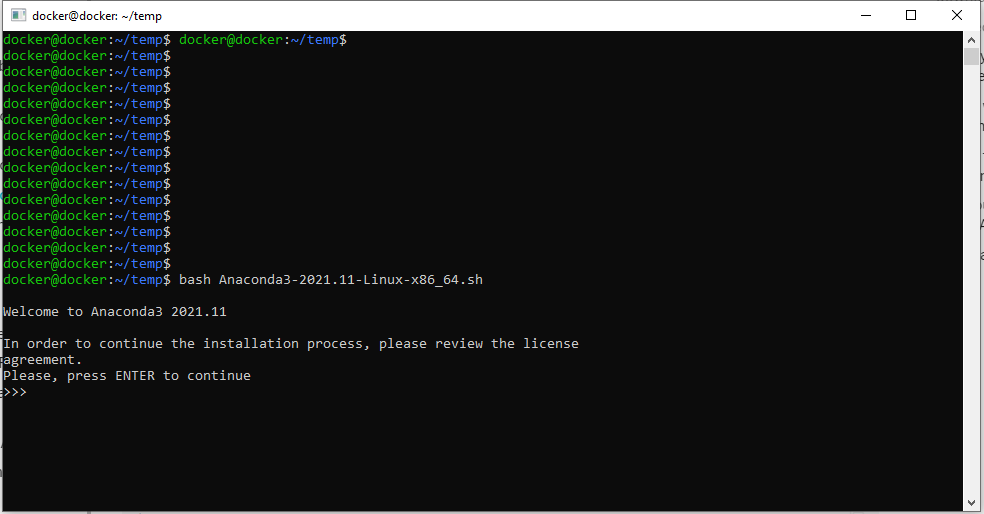
\includegraphics[scale=0.5]{figures/instalasi-anaconda-linux/step6}}
        \caption{Instalasi Anaconda Linux: Step 6}
\end{figure}
\item jika muncul gambar dibawah ini
\begin{figure}[H]
        \centerline{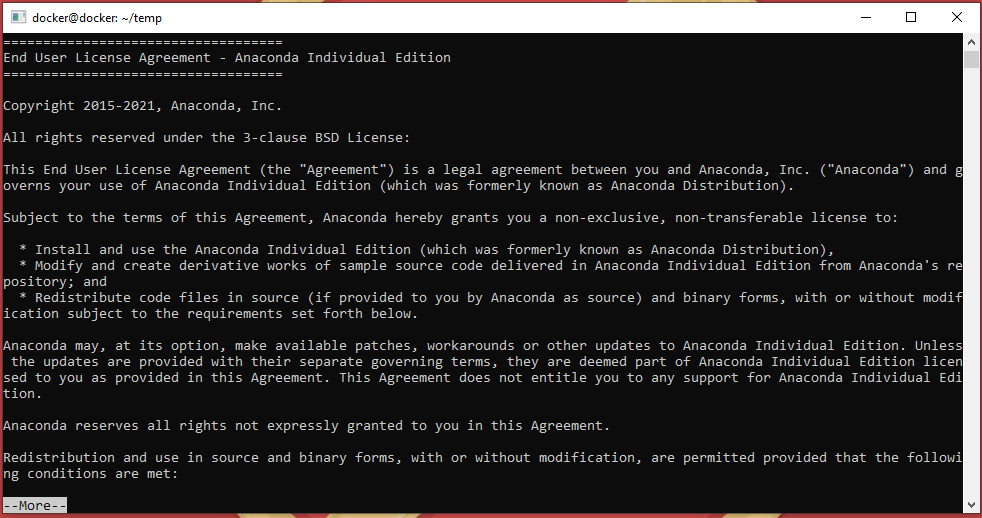
\includegraphics[scale=0.5]{figures/instalasi-anaconda-linux/step7}}
        \caption{Instalasi Anaconda Linux: Step 7}
\end{figure}
\item tekan dan tahan Enter sampai muncul gambar dibawah ini, lalu ketik yes, tekan enter
\begin{figure}[H]
        \centerline{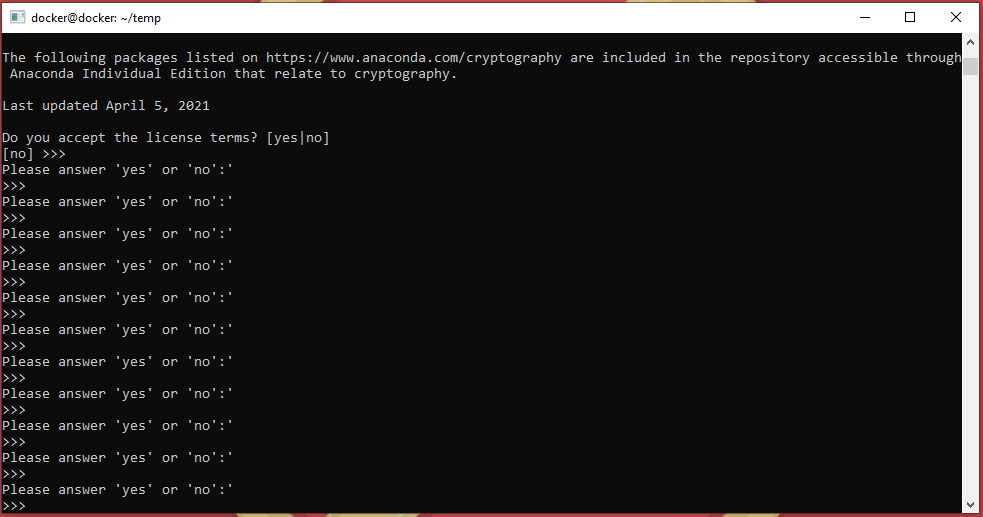
\includegraphics[scale=0.5]{figures/instalasi-anaconda-linux/step8}}
        \caption{Instalasi Anaconda Linux: Step 8}
\end{figure}
\item jika sudah seperti gambar dibawah, tekan enter
\begin{figure}[H]
        \centerline{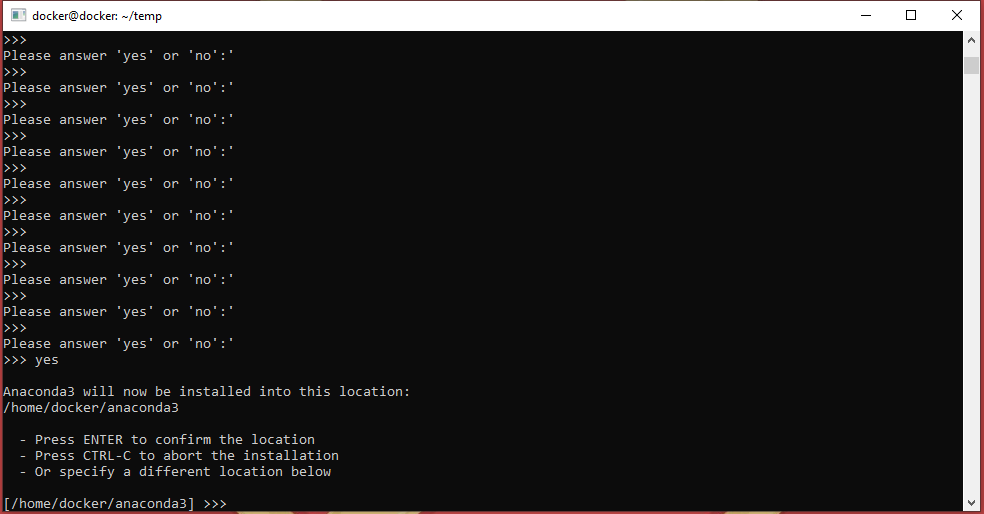
\includegraphics[scale=0.5]{figures/instalasi-anaconda-linux/step9}}
        \caption{Instalasi Anaconda Linux: Step 9}
\end{figure}
\item tunggu hingga proses selesai
\begin{figure}[H]
        \centerline{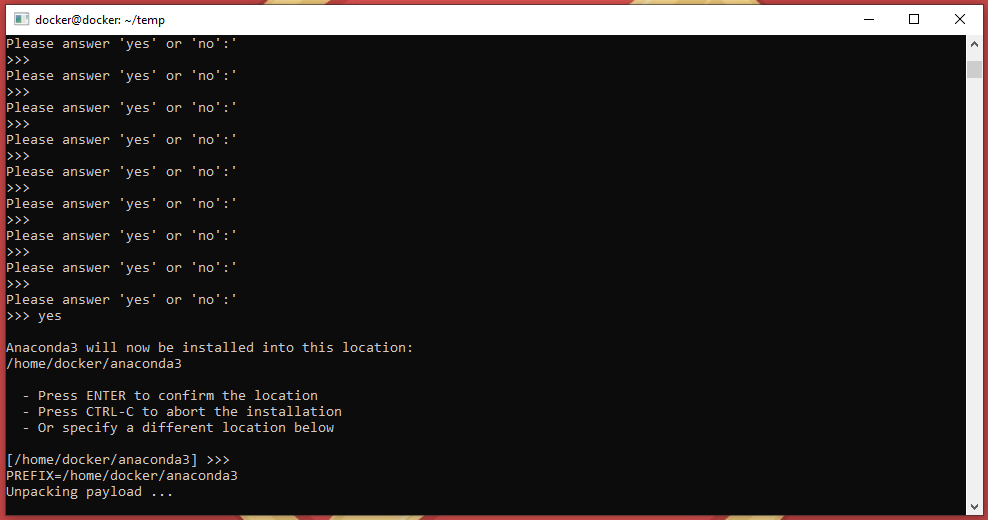
\includegraphics[scale=0.5]{figures/instalasi-anaconda-linux/step10}}
        \caption{Instalasi Anaconda Linux: Step 10}
\end{figure}
\item jika sudah selesai instalasi, ketikkan perintah berikut \textbf{export PYTHONPATH=\$PYTHONPATH:\textit{file path anaconda}} seperti dibawah ini, lalu tekan enter
\begin{figure}[H]
        \centerline{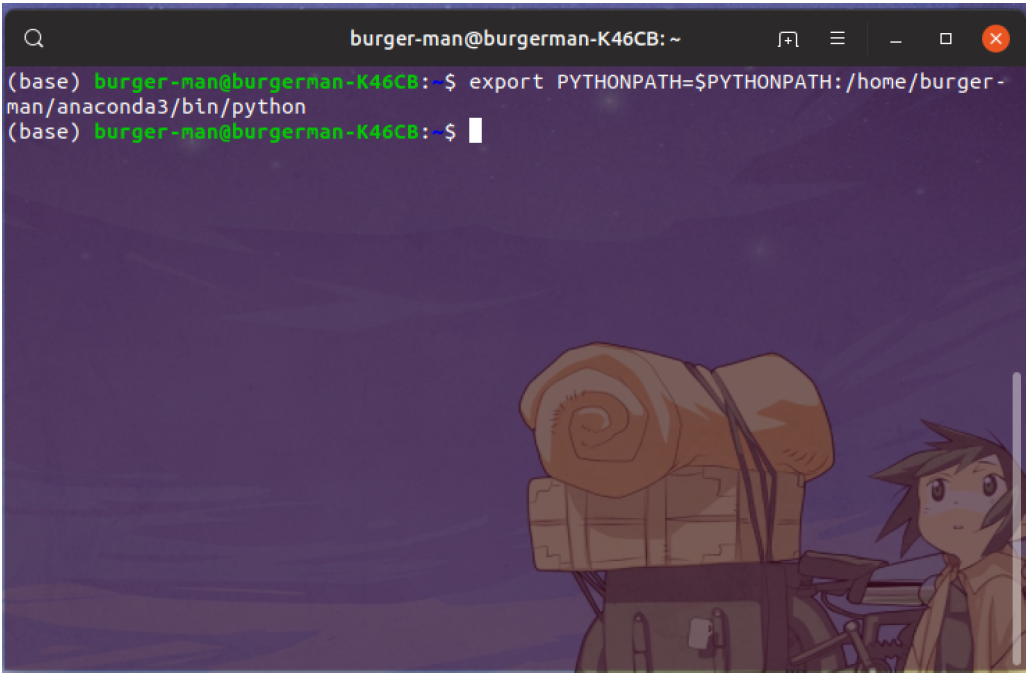
\includegraphics[scale=0.5]{figures/instalasi-anaconda-linux/step11}}
        \caption{Instalasi Anaconda Linux: Step 11}
\end{figure}
\end{enumerate}



\subsection{Windows}
Untuk instalasi python terdapat 2 cara yaitu menggunakan Python langsung atau menggunakan Anaconda

\subsubsection{Python}
\begin{enumerate}
\item Buka browser, kunjungi \url{http://www.python.org/downloads/windows/}
\item Buka (klik 2x) file installer python yang baru saja di download, lalu akan muncul seperti gambar dibawah ini.
\begin{figure}[H]
        \centerline{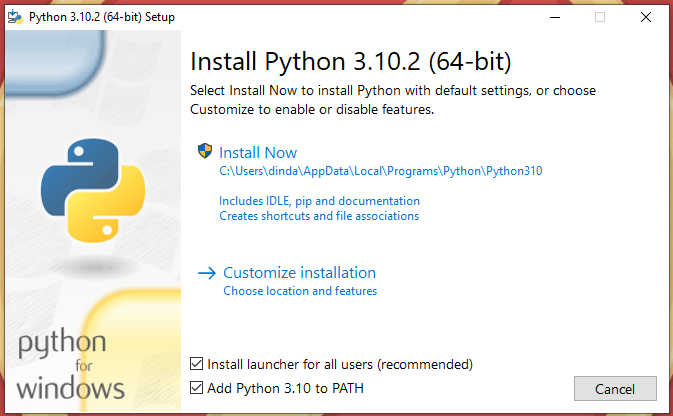
\includegraphics[scale=0.75]{figures/instalasi-python-windows/step1}}
        \caption{Instalasi Python Windows: Step 1}
\end{figure}
\item Pastikan sudah seperti gambar diatas, lalu klik tombol \textbf{Install Now}
\item Lalu akan muncul proses instalasi, tunggu sampai selesai.
\begin{figure}[H]
        \centerline{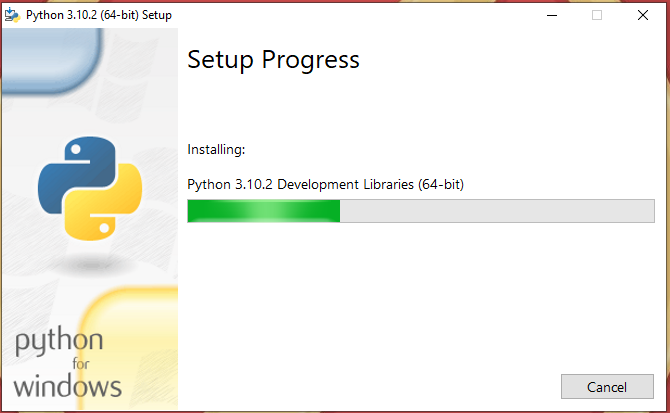
\includegraphics[scale=0.75]{figures/instalasi-python-windows/step2}}
        \caption{Instalasi Python Windows: Step 2}
\end{figure}
\item Jika sudah selesai akan muncul seperti gambar dibawah ini.
\begin{figure}[H]
        \centerline{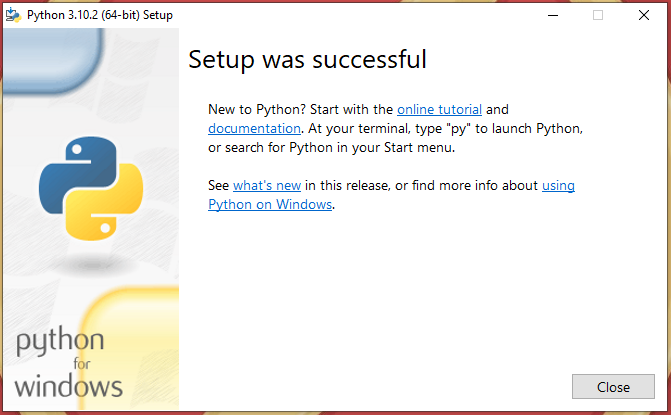
\includegraphics[scale=0.75]{figures/instalasi-python-windows/step3}}
        \caption{Instalasi Python Windows: Step 3}
\end{figure}
\end{enumerate}

\subsubsection{Anaconda}
\begin{enumerate}
\item Buka browser, kunjungi \url{https://www.anaconda.com/products/individual}, lalu download file Installer Anaconda sesuai Bit komputer/laptop anda.
\item Jika sudah download, klik (2x) filenya dan akan muncul seperti gambar dibawah ini.
\begin{figure}[H]
        \centerline{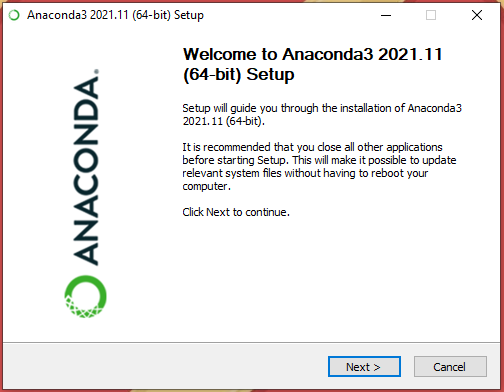
\includegraphics[scale=0.75]{figures/instalasi-anaconda-windows/step1}}
        \label{instalanacondawindowsstep1}
\end{figure}
\item Klik next setelah itu akan muncul seperti gambar dibawah ini.
\begin{figure}[H]
        \centerline{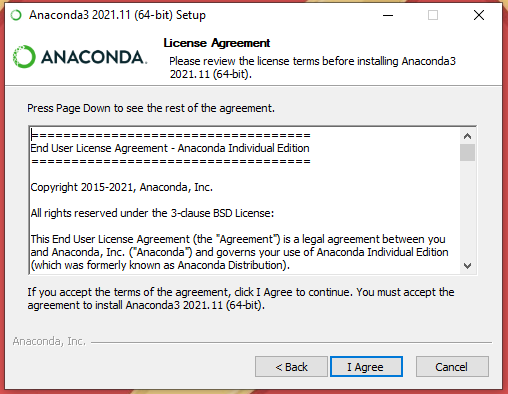
\includegraphics[scale=0.75]{figures/instalasi-anaconda-windows/step2}}
        \label{instalanacondawindowsstep2}
\end{figure}
\item klik I Agree, lalu akan muncul gambar dibawah ini.
\begin{figure}[H]
        \centerline{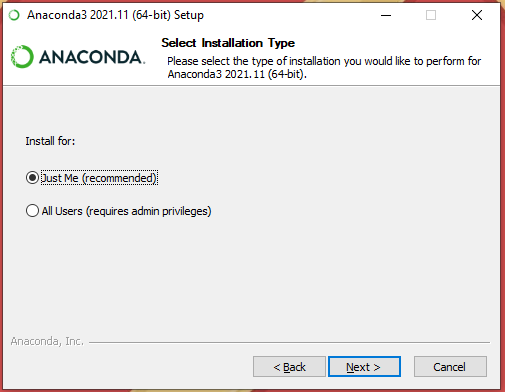
\includegraphics[scale=0.75]{figures/instalasi-anaconda-windows/step3}}
        \label{instalanacondawindowsstep3}
\end{figure}
\item lalu ada pilihan Just Me atau All Users, disini boleh bebas pilih yang mana saja, disini saya memilih Just Me karena direkomendasikan oleh Anacondanya, jika sudah memilih langsung klik next
\begin{figure}[H]
        \centerline{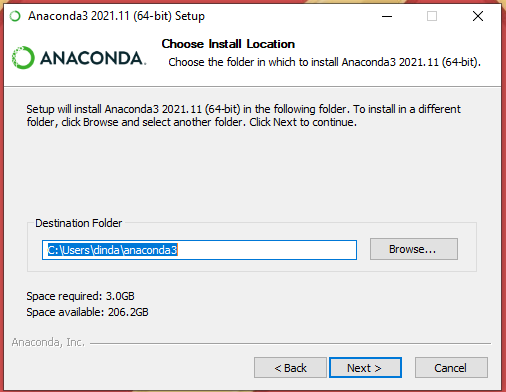
\includegraphics[scale=0.75]{figures/instalasi-anaconda-windows/step4}}
        \label{instalanacondawindowsstep4}
\end{figure}
\item setelah itu muncul destination folder adalah lokasi dimana ekstraksi file Anaconda akan diletakkan dimana, disini saya membiarkan seperti yang sudah diset default oleh Anaconda, klik next
\begin{figure}[H]
        \centerline{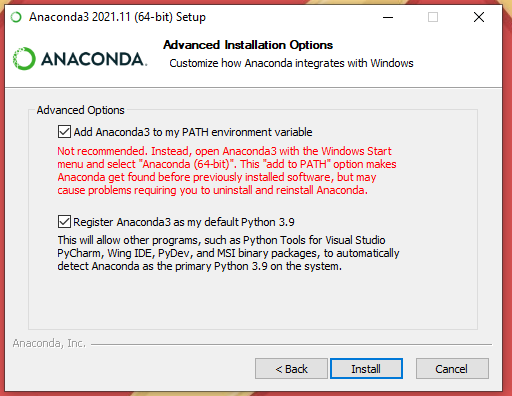
\includegraphics[scale=0.75]{figures/instalasi-anaconda-windows/step5}}
        \label{instalanacondawindowsstep5}
\end{figure}
\item setelah itu muncuk Menu Advanced Options, disini saya mencentang option Add Anaconda3 to my PATH environtment variabel, setelah itu klik install
\begin{figure}[H]
        \centerline{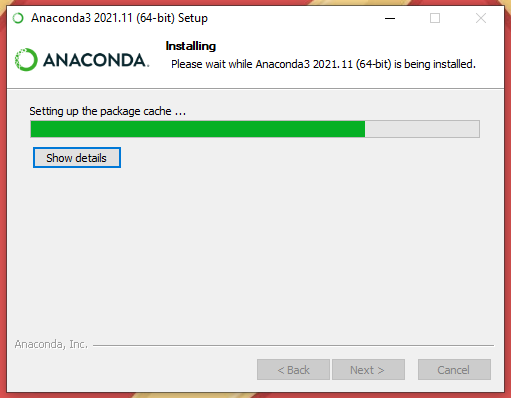
\includegraphics[scale=0.75]{figures/instalasi-anaconda-windows/step6}}
        \label{instalanacondawindowsstep6}
\end{figure}
\item tunggu proses instalasi hingga selesai
\begin{figure}[H]
        \centerline{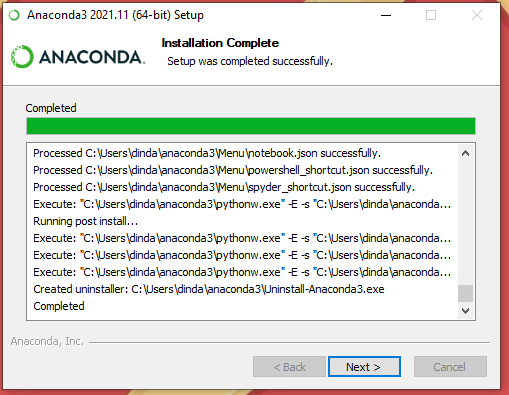
\includegraphics[scale=0.75]{figures/instalasi-anaconda-windows/step7}}
        \caption{Instalasi Anaconda Windows: Step 7}
\end{figure}
\item jika sudah muncul tulisan \textbf{Completed}, klik Next
\begin{figure}[H]
        \centerline{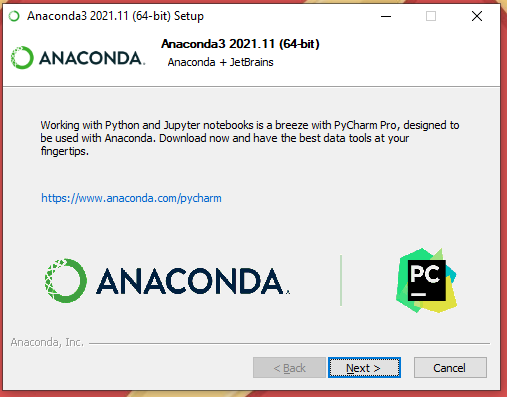
\includegraphics[scale=0.75]{figures/instalasi-anaconda-windows/step8}}
        \caption{Instalasi Anaconda Windows: Step 8}
\end{figure}
\item instalasi anaconda di windows 10 sudah selesai, klik next
\begin{figure}[H]
        \centerline{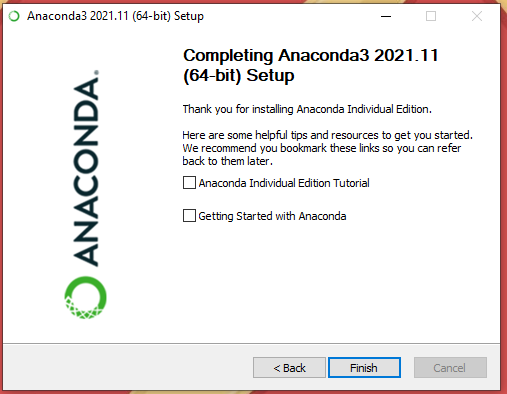
\includegraphics[scale=0.75]{figures/instalasi-anaconda-windows/step9}}
        \caption{Instalasi Anaconda Windows: Step 9}
\end{figure}
\item jika ingin mengunjungi website anaconda dan membaca manual secara lengkap boleh di centang kedua opsinya dan klik Finish, disini saya tidak mencentang kedua opsi.
\end{enumerate}

\section{Menjalankan Python}
Untuk menjalankan Python ada banyak cara yang bisa dilakukan. Anda bisa menggunakan \textit{shell}, terminal atau menggunakan IDE (Integrated Development Environment). Di bawah ini adalah langkah-langkah menjalankan Python dengan cara yang paling mudah.

\subsection{Linux}
\begin{enumerate}
\item Buka terminal CTRL + ALT + T
\begin{figure}[H]
        \centerline{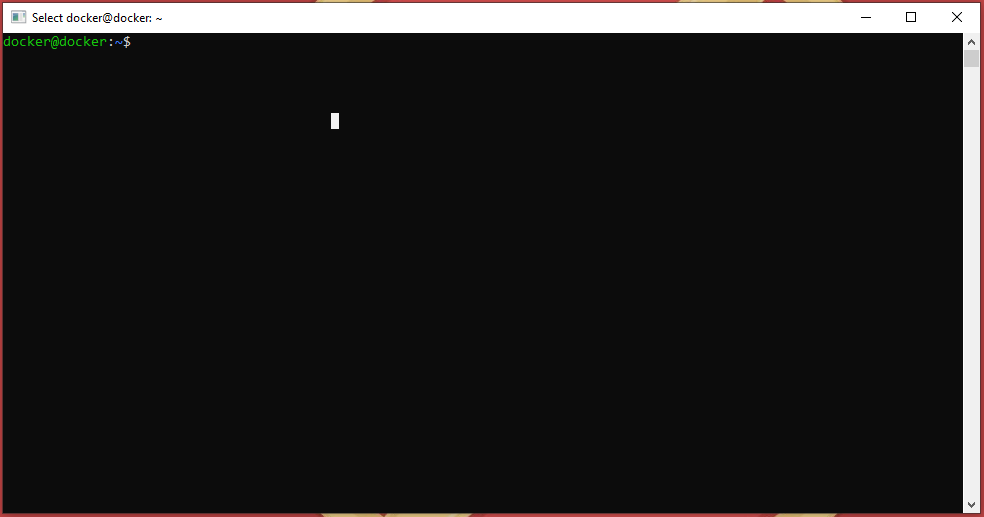
\includegraphics[scale=0.5]{figures/menjalankan-python-linux/step1}}
        \caption{Menjalankan Python Linux: Step 1}
\end{figure}
\item ketik \textbf{python3} lalu tekan enter
\begin{figure}[H]
        \centerline{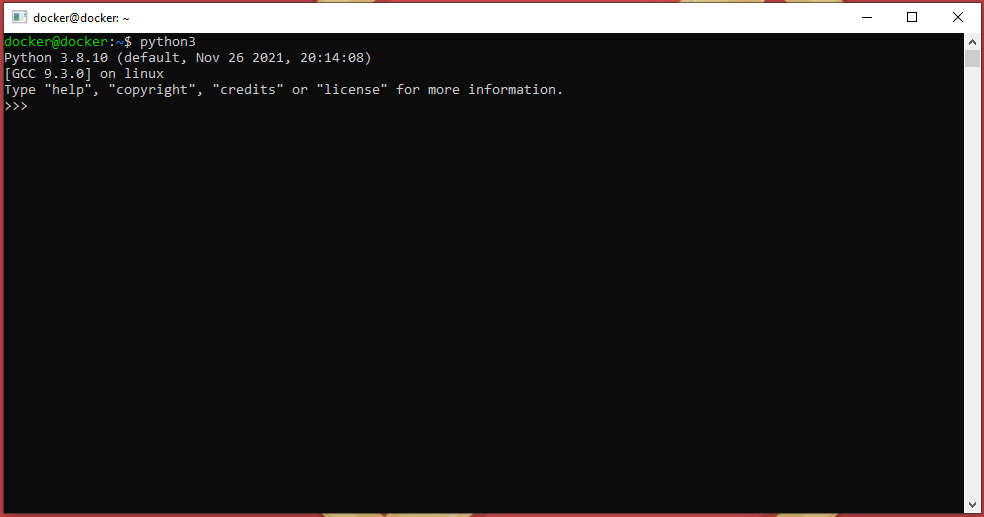
\includegraphics[scale=0.5]{figures/menjalankan-python-linux/step2}}
        \caption{Menjalankan Python Linux: Step 2}
\end{figure}
\item ketik \textbf{print("hello world")} tekan enter
\begin{figure}[H]
        \centerline{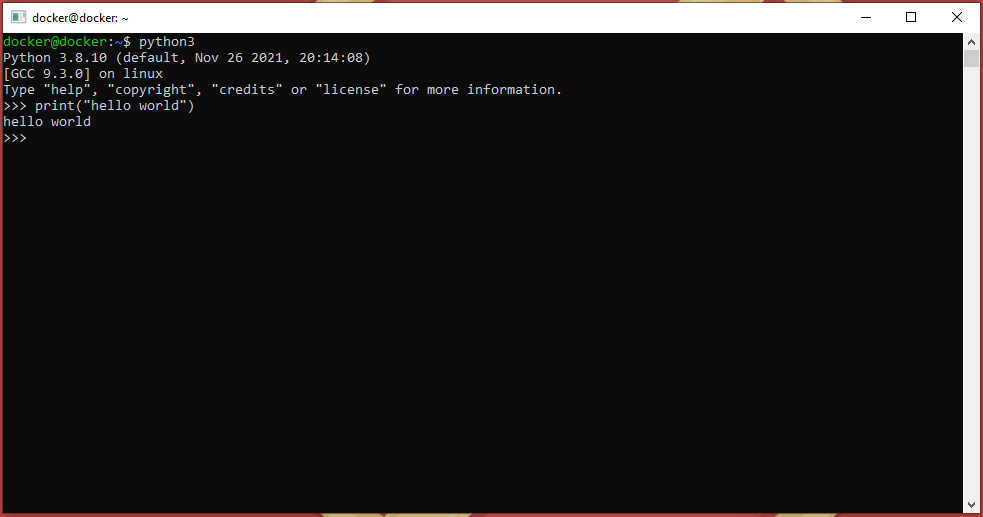
\includegraphics[scale=0.5]{figures/menjalankan-python-linux/step3}}
        \caption{Menjalankan Python Linux: Step 3}
\end{figure}
\item selamat anda sudah berhasil menjalankan program python3
\item jika ingin keluar dari shell python3 bisa dengan mengetik \textbf{exit()} lalu enter
\begin{figure}[H]
        \centerline{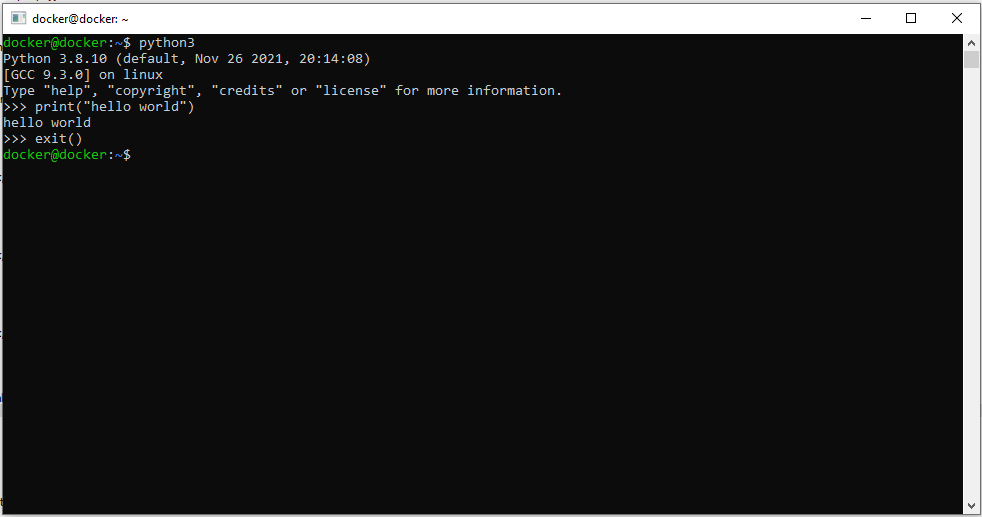
\includegraphics[scale=0.5]{figures/menjalankan-python-linux/step4}}
        \caption{Menjalankan Python Linux: Step 4}
\end{figure}
\end{enumerate}

\textit{atau}

\begin{enumerate}
\item Gunakan teks editor, misalnya \textbf{nano cetak.py}
\begin{figure}[H]
        \centerline{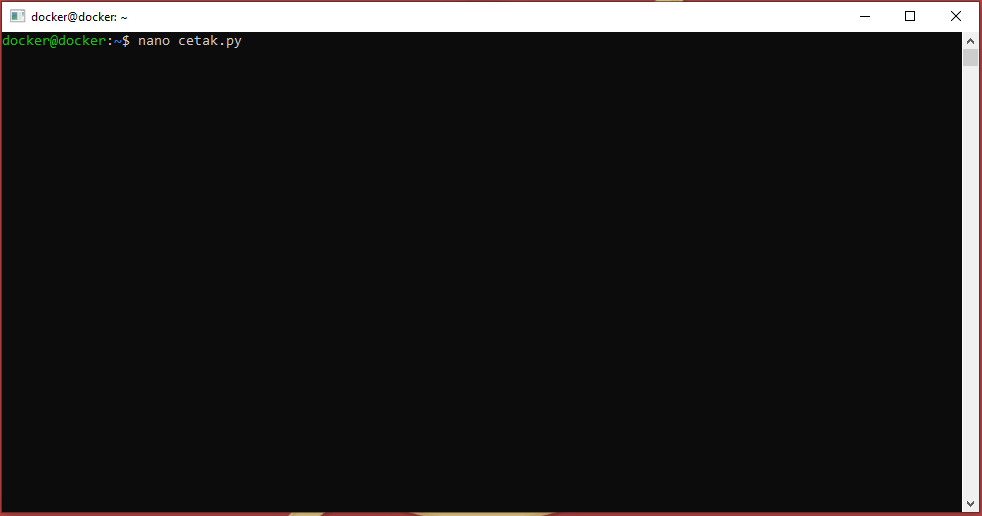
\includegraphics[scale=0.5]{figures/menjalankan-python-linux-with-nano/step1}}
        \caption{Menjalankan Python Linux dengan Teks Editor: Step 1}
\end{figure}
\item ketik \textbf{print("Selamat datang di Python")}
\begin{figure}[H]
        \centerline{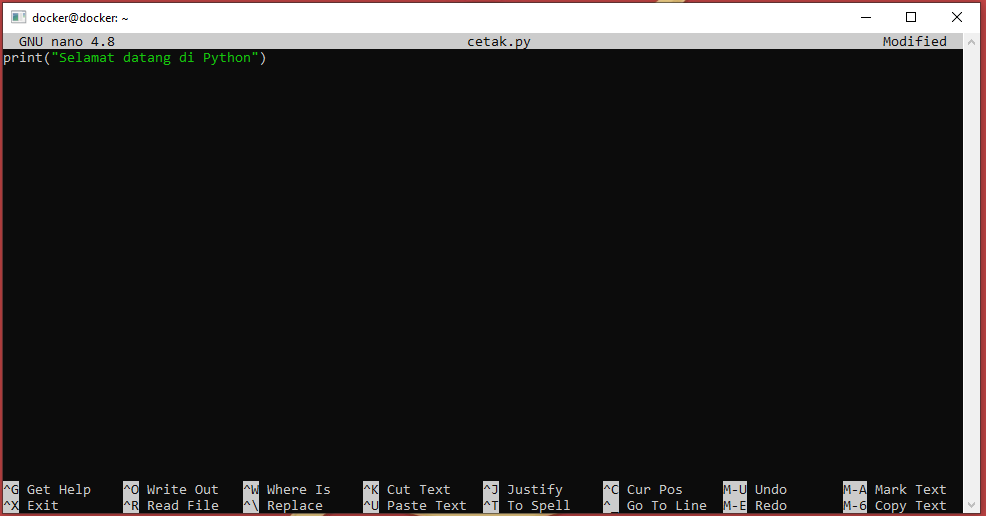
\includegraphics[scale=0.5]{figures/menjalankan-python-linux-with-nano/step2}}
        \caption{Menjalankan Python Linux dengan Teks Editor: Step 2}
\end{figure}
\item lalu tekan tombol CTRL + X
\begin{figure}[H]
        \centerline{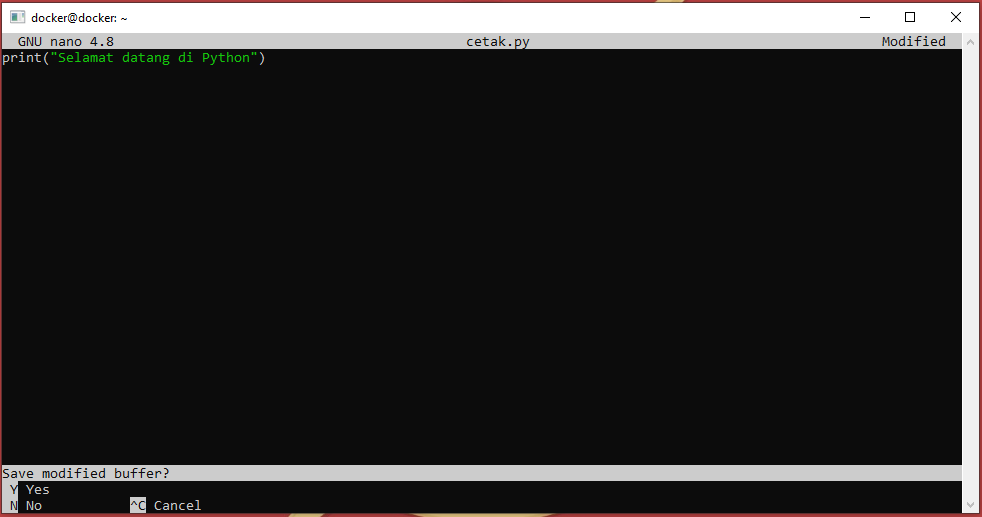
\includegraphics[scale=0.5]{figures/menjalankan-python-linux-with-nano/step3}}
        \caption{Menjalankan Python Linux dengan Teks Editor: Step 3}
\end{figure}
\item setelah itu tekan tombol \textbf{y}
\begin{figure}[H]
        \centerline{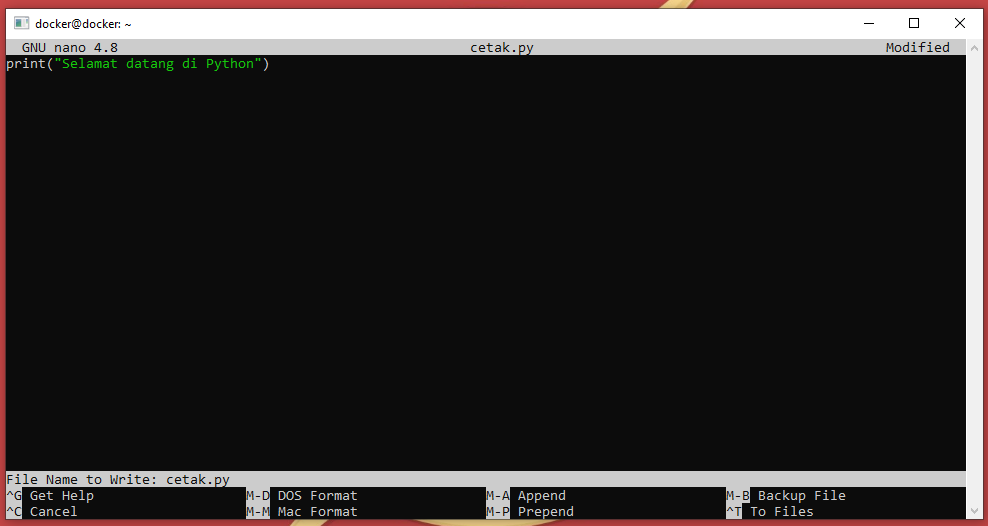
\includegraphics[scale=0.5]{figures/menjalankan-python-linux-with-nano/step4}}
        \caption{Menjalankan Python Linux dengan Teks Editor: Step 4}
\end{figure}
\item lalu tekan Enter
\begin{figure}[H]
        \centerline{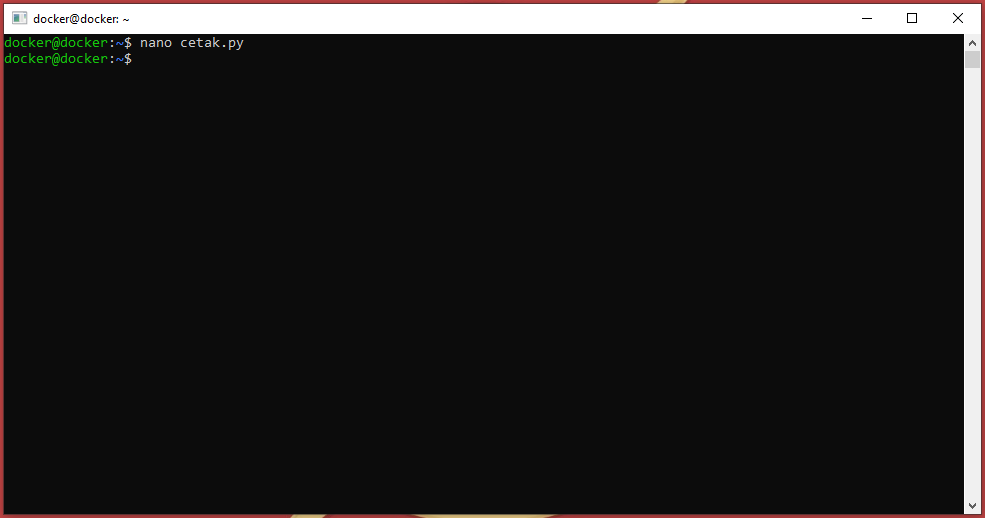
\includegraphics[scale=0.5]{figures/menjalankan-python-linux-with-nano/step5}}
        \caption{Menjalankan Python Linux dengan Teks Editor: Step 5}
\end{figure}
\item lalu ketikkan \textbf{python3 cetak.py}
\begin{figure}[H]
        \centerline{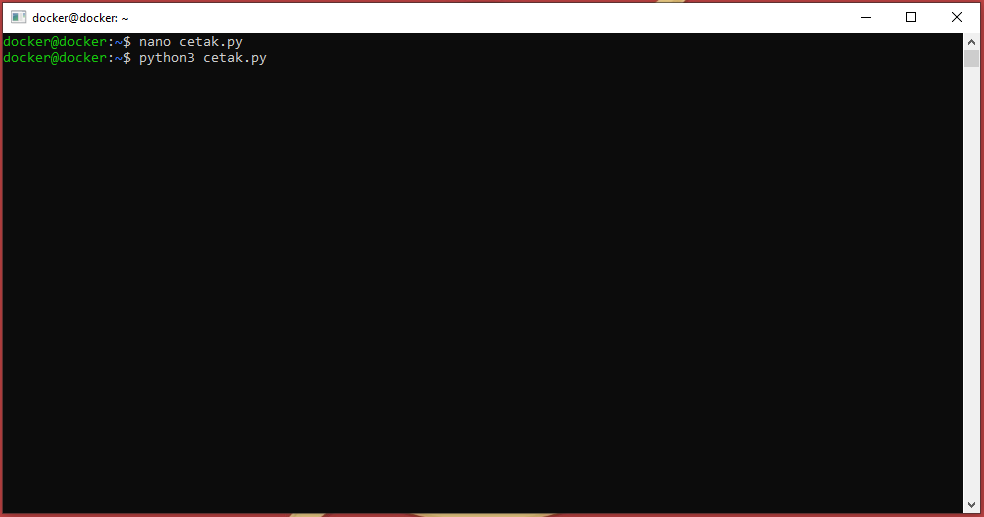
\includegraphics[scale=0.5]{figures/menjalankan-python-linux-with-nano/step6}}
        \caption{Menjalankan Python Linux dengan Teks Editor: Step 6}
\end{figure}
\item lalu tekan Enter
\begin{figure}[H]
        \centerline{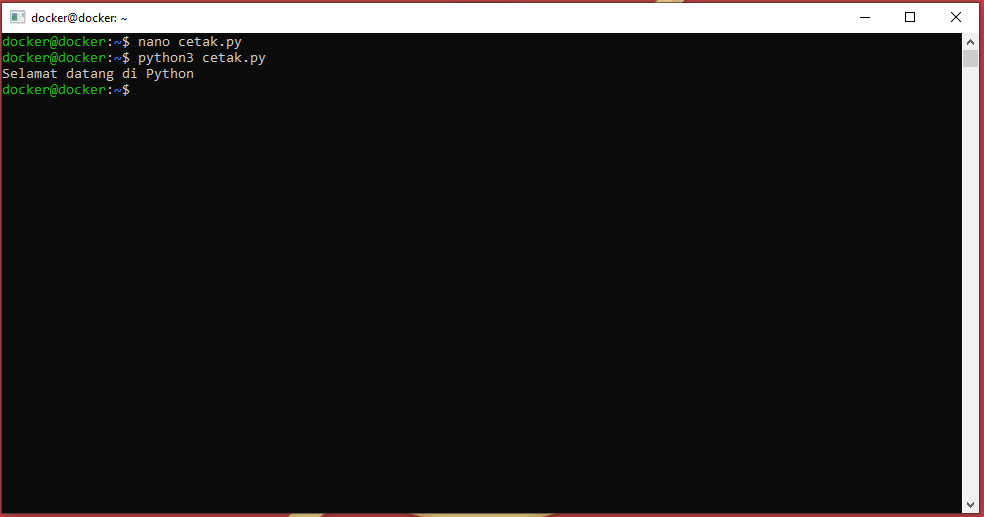
\includegraphics[scale=0.5]{figures/menjalankan-python-linux-with-nano/step7}}
        \caption{Menjalankan Python Linux dengan Teks Editor: Step 7}
\end{figure}
\end{enumerate}

\subsection{Windows}
\subsubsection{Menggunakan Shell}
\begin{enumerate}
\item Buka IDLE (python shell di windows), Anda bisa mencarinya di tombol START.
\item Tuliskan script Python Anda, contoh: print("Selamat datang di Python"). jika sudah tekan tombol ENTER, dan script Python akan dijalankan/eksekusi.
\begin{figure}[H]
        \centerline{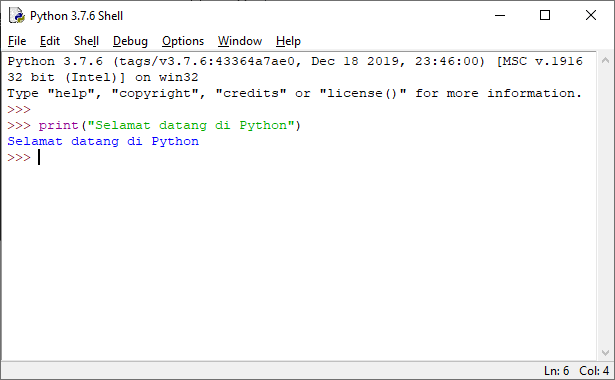
\includegraphics[scale=0.75]{figures/menjalankan-python-windows/step1}}
        \caption{Menjalankan Python Windows}
        \label{windowsshellpython}
\end{figure}
\item Untuk keluar dari Python shell ketik exit()
\end{enumerate}

\subsubsection{Menggunakan Script Editor}
\begin{enumerate}
\item Untuk menjalankan script yang disimpan dalam file, buka IDLE (python shell di windows), Anda bisa mencarinya di tombol START.
\item Klik menu File - New File
\item Tulis script Python pada window yang muncul, contoh:
\begin{lstlisting}[language=Python]
print("Belajar Python")
\end{lstlisting}
\item Simpan script lewat menu File - Save
\item Jalankan program dengan klik menu Run - Run Module
\end{enumerate}

\section{Hello World}
Syntax bahasa Python hampir sama dengan bahasa pemrograman pada umumnya seperti Java atau PHP.

\subsection{Syntax Dasar}
Dibawah ini adalah contoh fungsi Python yang digunakan untuk mencetak. Di Python untuk mencetak cukup gunakan fungsi print() , dimana sesuatu yang akan dicetak harus diletakkan diantara kurung buka dan kurung tutup, bahkan di Python versi 2.x Anda tidak harus menggunakan tanda kurung kurawal, cukup pisahkan dengan spasi. Jika ingin mencetak tipe data String langsung, Anda harus memasukanya ke dalam tanda kutip terlebih dahulu.
\begin{lstlisting}[language=Python]
print("Hello World")
\end{lstlisting}
Saat anda menjalankan script diatas, Anda akan melihat output berupa text Hello World.

\subsection{Python Case Sensitivity}
Python bersifat case sensitif, ini artinya huruf besar dan huruf kecil memiliki perbedaan. Sebagai contoh jika Anda menggunakan fungsi print dengan huruf kecil print() akan berhasil. Lain hal jika anda menggunakan huruf kapital Print() atau PRINT() , akan muncul pesan error. Aturan ini berlaku untuk nama variabel ataupun fungsi-fungsi lainnya.

\section{Komentar Python}
Komentar (comment) adalah kode di dalam script Python yang tidak dieksekusi atau tidak dijalankan mesin. Komentar hanya digunakan untuk menandai atau memberikan keterangan tertulis pada script. Komentar biasa digunakan untuk membiarkan orang lain memahami apa yang dilakukan script. atau untuk mengingatkan kepada programmer sendiri jika suatu saat kembali mengedit script tersebut. Untuk menggunakan komentar anda cukup menulis tanda pagar \#, diikuti dengan komentar Anda. Dibawah ini adalah contoh penggunaan komentar pada Python.
\lstinputlisting[caption=Python Comment, language=Python]{src/komentar.py}
Saat anda menjalankan script diatas, Anda akan melihat output berupa Hello World, Budi dan 123, karena tulisan/komentar yang ditulis tidak dieksekusi.

\section{Tipe Data Python}
Tipe data adalah suatu media atau memori pada komputer yang digunakan untuk menampung informasi. Python sendiri mempunyai tipe data yang cukup unik bila kita bandingkan dengan bahasa pemrograman yang lain. Berikut adalah tipe data dari bahasa pemrograman Python :

\begin{center}
\begin{tabular}{ | m{2cm} | m{2cm} | m{7cm} | }
\hline
Tipe Data & Contoh & Penjelasan \\
\hline
Boolean & \textbf{True} atau \textbf{False} & Menyatakan benar \textbf{True} yang bernilai \textbf{1}, atau salah \textbf{False} yang bernilai \textbf{0} \\
\hline
String & "Ayo belajar Python" & Menyatakan karakter/kalimat bisa berupa huruf angka, dll (diapit tanda " atau ') \\
\hline
Integer & 10 atau 100 & Menyatakan bilangan bulat \\
\hline
Float & 3.14 atau 1.22 & Menyatakan bilangan yang mempunyai koma \\
\hline
Hexadecimal & 9a atau 1d3 & Menyatakan bilangan dalam format heksa (bilangan berbasis 16) \\
\hline
Complex & 1 + 5j & Menyatakan pasangan angka real dan imajiner \\
\hline
List & ['tri', 'angga', 'dio', 'simamora'] atau [1, 2, 3, 4] & Data untaian yang menyimpan berbagai tipe data dan isinya bisa diubah atau modifikasi \\
\hline
Tuple & ('tri', 'angga', 'dio', 'simamora') atau (1, 2, 3, 4) & Data untaian yang menyimpan berbagai tipe data dan isinya tidak bisa diubah atau modifikasi \\
\hline
Dictionary & \{'nama': 'tri angga dio simamora'\} & Data untaian yang menyimpan berbagai tipe data berupa pasangan key dan value \\
\hline
\end{tabular}
\end{center}

Untuk mencoba berbagai macam tipe data, silahkan coba script Python dibawah ini.
\lstinputlisting[caption=Python Tipe Data, language=Python]{src/tipe_data.py}

\section{Variabel Python}
Variabel adalah lokasi memori yang dicadangkan untuk menyimpan nilai-nilai. Ini berarti bahwa ketika Anda membuat sebuah variabel Anda memesan beberapa ruang di memori. Variabel menyimpan data yang dilakukan selama program dieksekusi, yang nantinya isi dari variabel tersebut dapat diubah oleh operasi - operasi tertentu pada program yang menggunakan variabel.

Variabel dapat menyimpan berbagai macam tipe data. Di dalam pemrograman Python, variabel mempunyai sifat yang dinamis, artinya variabel Python tidak perlu didekralasikan tipe data tertentu dan variabel Python dapat diubah saat program dijalankan.

Penulisan variabel Python sendiri juga memiliki aturan tertentu, yaitu :

\begin{enumerate}
\item Karakter pertama harus berupa huruf atau garis bawah/underscore \textbf{\_}
\item Karakter selanjutnya dapat berupa huruf, garis bawah/underscore \textbf{\_} atau angka
\item Karakter pada nama variabel bersifat sensitif (case-sensitif). Artinya huruf kecil dan huruf besar dibedakan. Sebagai contoh, \textbf{namaDepan} dan \textbf{namadepan} adalah variabel yang berbeda.
\end{enumerate}

Untuk mulai membuat variabel di Python caranya sangat mudah, Anda cukup menuliskan variabel lalu mengisinya dengan suatu nilai dengan cara menambahkan tanda sama dengan \textbf{=} diikuti dengan nilai yang ingin dimasukan.

Dibawah ini adalah contoh penggunaan variabel dalam bahasa pemrograman Python
\lstinputlisting[caption=Python Variabel, language=Python]{src/variabel.py}

\section{Operator Python}
Operator adalah konstruksi yang dapat memanipulasi nilai dari operan. Sebagai contoh operasi 3 + 2 = 5. Disini 3 dan 2 adalah operan dan + adalah operator. Bahasa pemrograman Python mendukung berbagai macam operator, diantaranya :


\subsection{Operator Aritmatika}
\begin{center}
\begin{tabular}{ | m{2cm} | m{2cm} | m{7cm} | }
\hline
Operator & Contoh & Penjelasan \\
\hline
Penjumlahan & 1 + 3 = 4 & Menjumlahkan nilai dari masing-masing operan atau bilangan \\
\hline
Pengurangan & 4 - 1 = 3 & Mengurangi nilai operan di sebelah kiri menggunakan operan di sebelah kanan \\
\hline
Perkalian & 2 * 4 = 8 & Mengalikan operan/bilangan \\
\hline
Pembagian & 10 / 5 = 2 & Untuk membagi operan di sebelah kiri menggunakan operan di sebelah kanan \\
\hline
Sisa Bagi (Modulo) & 11 \% 2 = 1 & Mendapatkan sisa pembagian dari operan di sebelah kiri operator ketika dibagi oleh operan di sebelah kanan \\
\hline
Pangkat & 8 ** 2 = 64 & Memangkatkan operan disebelah kiri operator dengan operan di sebelah kanan operator \\
\hline
Pembagian Bulat & 10 // 3 = 3 & Sama seperti pembagian. Hanya saja angka dibelakang koma dihilangkan \\
\hline
\end{tabular}
\end{center}
Dibawah ini adalah contoh penggunaan Operator Aritmatika dalam bahasa pemrograman Python
\lstinputlisting[caption=Python Operator Aritmatika, language=Python]{src/aritmatika.py}

\subsection{Operator Perbandingan}
\begin{center}
\begin{tabular}{ | m{2cm} | m{2cm} | m{7cm} | }
\hline
Operator & Contoh & Penjelasan \\
\hline
Sama dengan & 1 == 1 & bernilai True Jika masing-masing operan memiliki nilai yang sama, maka kondisi bernilai benar atau True. \\
\hline
Tidak sama dengan & 2 != 2 & bernilai False Akan menghasilkan nilai kebalikan dari kondisi sebenarnya. \\
\hline
Tidak sama dengan & 2 \texttt{<>} 2 & bernilai False Akan menghasilkan nilai kebalikan dari kondisi sebenarnya. \\
\hline
Lebih besar dari & 5 \texttt{>} 3 & bernilai True Jika nilai operan kiri lebih besar dari nilai operan kanan, maka kondisi menjadi benar. \\
\hline
Lebih kecil dari & 5 \texttt{<} 3 & bernilai True Jika nilai operan kiri lebih kecil dari nilai operan kanan, maka kondisi menjadi benar. \\
\hline
Lebih besar atau sama dengan & 5 \texttt{>}= 3 & bernilai True Jika nilai operan kiri lebih besar dari nilai operan kanan, atau sama, maka kondisi menjadi benar. \\
\hline
Lebih kecil atau sama dengan & 5 \texttt{<}= 3 & bernilai True Jika nilai operan kiri lebih kecil dari nilai operan kanan, atau sama, maka kondisi menjadi benar. \\
\hline
\end{tabular}
\end{center}

\subsection{Operator Penugasan}
Operator penugasan digunakan untuk memberikan atau memodifikasi nilai ke dalam sebuah variabel.
\begin{center}
\begin{tabular}{ | m{2cm} | m{2cm} | m{7cm} | }
\hline
Operator & Contoh & Penjelasan \\
\hline
Sama dengan & a = 1 & Memberikan nilai di kanan ke dalam variabel yang berada di sebelah kiri. \\
\hline
Tambah sama dengann & a += 2 & Memberikan nilai variabel dengan nilai variabel itu sendiri ditambah dengan nilai di sebelah kanan. \\
\hline
Kurang sama dengan & a -= 2 & Memberikan nilai variabel dengan nilai variabel itu sendiri dikurangi dengan nilai di sebelah kanan. \\
\hline
Kali sama dengan & a *= 2 & Memberikan nilai variabel dengan nilai variabel itu sendiri dikali dengan nilai di sebelah kanan. \\
\hline
Bagi sama dengan & a /= 4 & Memberikan nilai variabel dengan nilai variabel itu sendiri dibagi dengan nilai di sebelah kanan. \\
\hline
Sisa bagi sama dengan & a \%= 3 & Memberikan nilai variabel dengan nilai variabel itu sendiri dibagi dengan nilai di sebelah kanan. Yang diambil nantinya adalah sisa baginya.\\
\hline
Pangkat sama dengan & a **= 3 & Memberikan nilai variabel dengan nilai variabel itu sendiri dipangkatkan dengan nilai di sebelah kanan. \\
\hline
Pembagian bulat sama dengan & a //= 3 & Membagi bulat operan sebelah kiri operator dengan operan sebelah kanan operator kemudian hasilnya diisikan ke operan sebelah kiri. \\
\hline
\end{tabular}
\end{center}

\subsection{Prioritas Eksekusi Operator di Python}
Dari semua operator diatas, masing-masing mempunyai urutan prioritas yang nantinya prioritas pertama akan dilakukan paling pertama, begitu seterusnya sampai dengan prioritas terakhir.
\begin{center}
\begin{tabular}{ | m{4cm} | m{4cm} | }
\hline
Operator & Keterangan \\
\hline
** & Aritmatika \\
\hline
~, +, - & Bitwise \\
\hline
*, /, \%, // & Aritmatika \\
\hline
+, - & Aritmatika \\
\hline
\texttt{>>}, \texttt{<<} & Bitwise \\
\hline
\& & Bitwise \\
\hline
\^, | & Bitwise \\
\hline
\texttt{<}=, \texttt{<}, \texttt{>}, \texttt{>}= & Perbandingan \\
\hline
\texttt{<>} , ==, != & Perbandingan \\
\hline
=, \%=, /=, //=, -=, +=, *=, **= & Penugasan \\
\hline
is, is not & Identitas \\
\hline
in, not in & Membership (Keanggotaan) \\
\hline
not, or, and & Logika \\
\hline
\end{tabular}
\end{center}


\section{Kondisi Python}

\subsection{Kondisi If}
Pengambilan keputusan (kondisi if) digunakan untuk mengantisipasi kondisi yang terjadi saat jalanya program dan menentukan tindakan apa yang akan diambil sesuai dengan kondisi. Pada python ada beberapa statement/kondisi diantaranya adalah if, else dan elif Kondisi if digunakan untuk mengeksekusi kode jika kondisi bernilai benar True. Jika kondisi bernilai salah False maka statement/kondisi if tidak akan di-eksekusi. Dibawah ini adalah contoh penggunaan kondisi if pada Python
\lstinputlisting[caption=Python Kondisi If, language=Python]{src/if.py}
Dari contoh diatas, jika program dijalankan maka akan mencetak string "Sembilan Lebih Besar Dari Angka Tujuh" sebanyak 1 kali yaitu pada if pertama. Di if kedua statement bernilai salah, jadi perintah print("Sembilan Lebih Besar Dari Angka Sepuluh") tidak akan dieksekusi.

\subsection{Kondisi If Else}
Pengambilan keputusan (kondisi if else) tidak hanya digunakan untuk menentukan tindakan apa yang akan diambil sesuai dengan kondisi, tetapi juga digunakan untuk menentukan tindakan apa yang akan diambil/dijalankan jika kondisi tidak sesuai. Pada python ada beberapa statement/kondisi diantaranya adalah if, else dan elif Kondisi if digunakan untuk mengeksekusi kode jika kondisi bernilai benar. Kondisi if else adalah kondisi dimana jika pernyataan benar True maka kode dalam if akan dieksekusi, tetapi jika bernilai salah False maka akan mengeksekusi kode di dalam else. Dibawah ini adalah contoh penggunaan kondisi if else pada Python
\lstinputlisting[caption=Python Kondisi If Else, language=Python]{src/ifelse.py}
Pada contoh diatas, jika program dijalankan maka akan mencetak string "Maaf Anda Tidak Lulus" karena pernyataan pada if bernilai False

\subsection{Kondisi Elif}
Pengambilan keputusan (kondisi if elif) merupakan lanjutan/percabangan logika dari “kondisi if”. Dengan elif kita bisa membuat kode program yang akan menyeleksi beberapa kemungkinan yang bisa terjadi. Hampir sama dengan kondisi “else”, bedanya kondisi “elif” bisa banyak dan tidak hanya satu.

Dibawah ini adalah contoh penggunaan kondisi elif pada Python
\lstinputlisting[caption=Python Kondisi Elif, language=Python]{src/elif.py}
Pada contoh diatas, jika program dijalankan maka akan mencetak string "Saya akan libur".

\section{Loop Python}
Secara umum, pernyataan pada bahasa pemrograman akan dieksekusi secara berurutan. Pernyataan pertama dalam sebuah fungsi dijalankan pertama, diikuti oleh yang kedua, dan seterusnya. Tetapi akan ada situasi dimana Anda harus menulis banyak kode, dimana kode tersebut sangat banyak. Jika dilakukan secara manual maka Anda hanya akan membuang-buang tenaga dengan menulis beratus-ratus bahkan beribu-ribu kode. Untuk itu Anda perlu menggunakan pengulangan di dalam bahasa pemrograman Python.

Di dalam bahasa pemrograman Python pengulangan dibagi menjadi 3 bagian, yaitu :
\begin{itemize}
\item While Loop
\item For Loop
\item Nested Loop
\end{itemize}


\subsection{While Loop}
Pengulangan While Loop di dalam bahasa pemrograman Python dieksesusi statement berkali-kali selama kondisi bernilai benar atau True.

Dibawah ini adalah contoh penggunaan pengulangan While Loop.
\lstinputlisting[caption=Python While Loop, language=Python]{src/whileloop.py}


\subsection{For Loop}
Pengulangan for pada Python memiliki kemampuan untuk mengulangi item dari urutan apapun, seperti list atau string.

Dibawah ini adalah contoh penggunaan pengulangan For Loop.
\lstinputlisting[caption=Python For Loop, language=Python]{src/forloop.py}


\subsection{Nested Loop}
Bahasa pemrograman Python memungkinkan penggunaan satu lingkaran di dalam loop lain. Bagian berikut menunjukkan beberapa contoh untuk menggambarkan konsep tersebut.

Dibawah ini adalah contoh penggunaan Nested Loop.
\lstinputlisting[caption=Python Nested Loop, language=Python]{src/nestedloop.py}


\section{Number Python}
Number adalah tipe data Python yang menyimpan nilai numerik. Number adalah tipe data yang tidak berubah. Ini berarti, mengubah nilai dari sejumlah tipe data akan menghasilkan objek yang baru dialokasikan.

Objek Number dibuat saat Anda memberikan nilai pada-nya. Sebagai contoh : angkaPertama = 1 angkaKedua = 33

Python mendukung beberapa tipe data Number diantaranya :
\begin{itemize}
\item Int
\item Float
\item Complex
\end{itemize}

Berikut ini adalah beberapa contoh dari Tipe data Number pada Python :

\begin{center}
\begin{tabular}{ | m{3cm} | m{3cm} | m{3cm} | }
\hline
Int & Float & Complex \\
\hline
20 & 0.1 & 3.14j \\
\hline
300 & 1.20 & 35.j \\
\hline
-13 & -41.2 & 3.12e-12j \\
\hline
020 & 32.23+e123 & .873j \\
\hline
-0103 & -92. & -.123+0J \\
\hline
-0x212 & -32.52e10 & 3e+123J \\
\hline
0x56 & 60.2-E13 & 4.31e-4j \\
\hline
\end{tabular}
\end{center}


\subsection{Konversi Tipe Data Number Python}
Pada Python Anda bisa mengkonversi tipe data dengan menggunakan fungsi. Dibawah ini adalah beberapa fungsi untuk mengkonversi tipe data number Python.
\begin{itemize}
\item int(x) untuk meng-konversi x menjadi plain integer.
\item long(x) untuk meng-konversi x menjadi long integer.
\item float(x) untuk meng-konversi x menjadi floating point number.
\item complex(x) untuk meng-konversi x menjadi complex number dengna real part x dan imaginary part zero.
\item complex(x, y) untuk meng-konversi x dan y menjadi complex number dengan real part x dan imaginary part y. x dan numeric expressions y.
\end{itemize}


\subsection{Fungsi Matematika Python}
Pada bahasa pemrograman Python terdapat fungsi untuk melakukan perhitungan matematis, berikut adalah daftarnya:
\begin{center}
\begin{tabular}{ | m{2cm} | m{2cm} | m{5cm} | }
\hline
Penjelasan & Penggunaan & Penjelasan \\
\hline
Absolute & abs(x) & Nilai absolut dari x:(positive) jarak antara x and 0. \\
\hline
Ceiling & ceil(x) & Ceiling dari x: integer terkecil yang kurang dari x. \\
\hline
Cmp & cmp(x, y) & -1 if x \texttt{<} y, 0 if x == y, or 1 if x \texttt{>} y. Tidak berlaku lagi dengan Python 3. Sebaliknya gunakan return (x\texttt{>}y)-(x \\
\hline
Eksponen & exp(x) & Nilai eksponen dari x: ex \\
\hline
Fabs & fabs(x) & Nilai absolut dari x. \\
\hline
Floor & floor(x) & Nilai dasar dari x: internet terbesar tidak lebih besar dari x. \\
\hline
Log & log(x) & Logaritma dari x, untuk x \texttt{>} 0. \\
\hline
Log 10 & log10(x) & Basis 10 logaritma dari x, untuk x \texttt{>} 0. \\
\hline
Max & max(x1, x2,...) & Argumen terbesar: Nilai terdekat dengan tak terhingga positif \\
\hline
Min & min(x1, x2,...) & Argumen terkecil: nilai yang paling mendekati tak berhingga negatif. \\
\hline
Modf & modf(x) & Bagian pecahan dan bilangan bulat dari x dalam tupel dua item. Kedua bagian memiliki tanda yang sama dengan x. Bagian integer dikembalikan sebagai float. \\
\hline
Pow & pow(x, y) & Nilai x ** y. \\
\hline
Round & round(x [,n]) & X dibulatkan menjadi n digit dari titik desimal. Putaran Python jauh dari nol sebagai tie-breaker: round (0.5) adalah 1.0 dan round (-0.5) adalah -1.0. \\
\hline
Akar Kuadrat & sqrt(x) & Akar kuadrat x untuk x \texttt{>} 0. \\
\hline
\end{tabular}
\end{center}

\subsection{Fungsi Nomor Acak Python}
Nomor acak digunakan untuk aplikasi permainan, simulasi, pengujian, keamanan, dan privasi. Python mencakup fungsi berikut yang umum digunakan. Berikut adalah daftarnya :
\subsection{Fungsi Matematika Python}
Pada bahasa pemrograman Python terdapat fungsi untuk melakukan perhitungan matematis, berikut adalah daftarnya:
\begin{center}
\begin{tabular}{ | m{2cm} | m{2cm} | m{5cm} | }
\hline
Penjelasan & Penggunaan & Penjelasan \\
\hline
Choice & choice(seq) & Item acak dari list, tuple, atau string. \\
\hline
RandRange & randrange ([start,] stop [,step]) & Elemen yang dipilih secara acak dari jangkauan (start, stop, step). \\
\hline
Random & random() & A random float r, sehingga 0 kurang dari atau sama dengan r dan r kurang dari 1 \\
\hline
Seed & seed([x]) & Menetapkan nilai awal integer yang digunakan dalam menghasilkan bilangan acak. Panggil fungsi ini sebelum memanggil fungsi modul acak lainnya. Tidak ada pengembalian \\
\hline
Shuffle & shuffle(lst) & Mengacak daftar dari daftar di tempat. Tidak ada pengembalian \\
\hline
Floor & floor(x) & The floor of x: the largest integer not greater than x. \\
\hline
Uniform & uniform(x, y) & Sebuah float acak r, sedemikian rupa sehingga x kurang dari atau sama dengan r dan r kurang dari y. \\
\hline
\end{tabular}
\end{center}

\subsection{Fungsi Trigonometri Python}
Python mencakup fungsi berikut yang melakukan perhitungan trigonometri. Berikut adalah daftarnya :
\begin{center}
\begin{tabular}{ | m{2cm} | m{2cm} | m{5cm} | }
\hline
Penjelasan & Penggunaan & Penjelasan \\
\hline
Acos & acos(x) & Kembalikan kosinus x, di radian.\\
\hline
Asin & asin(x) & Kembalikan busur sinus x, dalam radian.\\
\hline
Atan & atan(x) & Kembalikan busur singgung x, di radian.\\
\hline
Atan 2 & atan2(y, x) & Kembali atan (y / x), di radian.\\
\hline
Kosinus & cos(x) & Kembalikan kosinus x radian.\\
\hline
Hypot & hypot(x, y) & Kembalikan norma Euclidean, sqrt (x * x + y * y).\\
\hline
Sin & sin(x) & Kembalikan sinus dari x radian.\\
\hline
Tan & tan(x) & Kembalikan tangen x radian.\\
\hline
Derajat & degrees(x) & Mengonversi sudut x dari radian ke derajat.\\
\hline
Radian & radians(x) & Mengonversi sudut x dari derajat ke radian.\\
\hline
\end{tabular}
\end{center}

\subsection{Konstanta Matematika Python}
Modul ini juga mendefinisikan dua konstanta matematika. Berikut adalah daftarnya :
\begin{center}
\begin{tabular}{ | m{2cm} | m{2cm} | m{5cm} | }
\hline
Penjelasan & Penggunaan & Penjelasan \\
\hline
Pi & pi & Konstanta Pi matematika\\
\hline
e & e & Konstanta e matematika\\
\hline
\end{tabular}
\end{center}

\section{String Python}
String adalah jenis yang paling populer di bahasa pemrograman. Kita bisa membuatnya hanya dengan melampirkan karakter dalam tanda kutip. Python memperlakukan tanda kutip tunggal sama dengan tanda kutip ganda. Membuat string semudah memberi nilai pada sebuah variabel.

Dibawah ini adalah contoh sederhana dari sebuah string pada bahasa pemrograman Python.
\begin{lstlisting}[language=Python]
hello = "Hello World" # hello adalah variabel yang diisi oleh string
print(hello)
\end{lstlisting}

\subsection{Mengakses Nilai dalam String}
Python tidak menggunakan tipe karakter titik koma ; Ini diperlakukan sebagai string dengan panjang satu, sehingga juga dianggap sebagai substring.

Untuk mengakses substring, gunakan tanda kurung siku untuk mengiris beserta indeks atau indeks untuk mendapatkan substring Anda. Sebagai contoh :
\begin{lstlisting}[language=Python]
hello = "Hello World"
print(hello[0])
\end{lstlisting}


\subsection{Mengupdate String}
Anda dapat “memperbarui” string yang ada dengan (kembali) menugaskan variabel ke string lain. Nilai baru dapat dikaitkan dengan nilai sebelumnya atau ke string yang sama sekali berbeda sama sekali. Sebagai contoh
\begin{lstlisting}[language=Python]
hello = "Hello World"
print ("Updated String :- ", hello[:6] + 'Python')
\end{lstlisting}

\subsection{Karakter Escape Python}
Dibawah ini adalah tabel dari daftar karakter escape atau karakter non-printable yang dapat diwakili/ditulis dengan awalan notasi backslash.
\begin{center}
\begin{tabular}{ | m{3cm} | m{3cm} | m{3cm} | }
\hline
Notasi Backslash & Karakter Hexa & Penjelasan \\
\hline
\textbackslash a & 0x07 & Bell atau alert \\
\hline
\textbackslash b & 0x08 & Backspace \\
\hline
\textbackslash cx & - & Control-x \\
\hline
\textbackslash C-x & - & Control-x\\
\hline
\textbackslash e & 0x1b & Escape\\
\hline
\textbackslash f & 0x0c & Formfeed\\
\hline
\textbackslash M-\textbackslash C-x & - & Meta-Control-x\\
\hline
\textbackslash n & 0x0a & Newline\\
\hline
\textbackslash nnn & - & Octal notation, dimana n berada di range 0.7\\
\hline
\textbackslash r & 0x0d & Carriage return\\
\hline
\textbackslash s & 0x20 & Space\\
\hline
\textbackslash t & 0x09 & Tab\\
\hline
\textbackslash v & 0x0b & Vertical tab\\
\hline
\textbackslash x & - & Character x\\
\hline
\textbackslash xnn & - & Notasi Hexadecimal, dimana n berada di range 0.9, a.f, atau A.F\\
\hline
\end{tabular}
\end{center}

\subsection{Operator Spesial String Python}
Asumsikan variabel string adalah ‘Belajar’ dan variabel b adalah ‘Python’, lalu dibawah ini adalah operator yang bisa dipakai pada kedua string di variabel tersebut. a = "Belajar" b = "Python"

Berikut adalah daftar operator spesial string pada Python :
\begin{center}
\begin{tabular}{ | m{2cm} | m{2cm} | m{5cm} | }
\hline
Operator & Contoh & Penjelasan \\
\hline
+ & a + b & akan menghasilkan BelajarPython Concatenation - Menambahkan nilai pada kedua sisi operator\\
\hline
* & a*2 & akan menghasilkan BelajarBelajar Pengulangan - Membuat string baru, menggabungkan beberapa salinan dari string yang sama\\
\hline
[] & a[1] & akan menghasilkan e Slice - Memberikan karakter dari indeks yang diberikan\\
\hline
[ : ] & a[1:4] & akan menghasilkan ela Range Slice - Memberikan karakter dari kisaran yang diberikan\\
\hline
in & B in a & akan menghasilkan 1 Keanggotaan - Mengembalikan nilai true jika ada karakter dalam string yang diberikan\\
\hline
not in & Z not in a & akan menghasilkan 1 Keanggotaan - Mengembalikan nilai true jika karakter tidak ada dalam string yang diberikan\\
\hline
r/R & print r’\textbackslash n’ prints \textbackslash n dan print R’ \textbackslash n’prints \textbackslash n Raw String - & Menekan arti aktual karakter Escape. Sintaks untuk string mentah sama persis dengan string biasa kecuali operator string mentah, huruf “r”, yang mendahului tanda petik. “R” bisa berupa huruf kecil (r) atau huruf besar (R) dan harus ditempatkan tepat sebelum tanda kutip pertama.\\
\hline
\% & & Format - Melakukan format String\\
\hline
\end{tabular}
\end{center}

\subsection{Operator Format String Python}
Salah satu fitur Python yang paling keren adalah format string operator \%. Operator ini unik untuk string dan membuat paket memiliki fungsi dari keluarga printf C () C. berikut adalah contoh sederhananya :
\begin{lstlisting}[language=Python]
print ("My name is %s and weight is %d kg!" % ('Andi', 21))
\end{lstlisting}

Berikut adalah daftar lengkap simbol yang bisa digunakan bersamaan dengan \% :
\begin{center}
\begin{tabular}{ | m{2cm} | m{5cm} | }
\hline
Operator & Penjelasan \\
\hline
\%c & character \\
\hline
\%s & Konversi string melalui str () sebelum memformat \\
\hline
\%i & Dianggap sebagai bilangan bulat desimal \\
\hline
\%d & Dianggap sebagai bilangan bulat desimal \\
\hline
\%u & Unsigned decimal integer \\
\hline
\%o & Bilangan bulat oktal \\
\hline
\%x & Bilangan bulat heksadesimal (huruf kecil) \\
\hline
\%X & Bilangan bulat heksadesimal (huruf besar) \\
\hline
\%e & Notasi eksponensial (dengan huruf kecil ‘e’) \\
\hline
\%E & Notasi eksponensial (dengan huruf besar ‘E’) \\
\hline
\%f & Bilangan real floating point \\
\hline
\%g & Yang lebih pendek dari\% f dan\% e \\
\hline
\%G & Lebih pendek dari\% f dan\% E \\
\hline
\end{tabular}
\end{center}

\subsection{Triple Quote Python}
Python triple quotes digunakan dengan membiarkan string untuk ditulis dalam beberapa baris, termasuk kata kerja NEWLINEs, TABs, dan karakter khusus lainnya. Sintaks untuk triple quotes terdiri dari tiga tanda kutip tunggal atau ganda ditulis berturut-turut : Berikut adalah contohnya :
\begin{lstlisting}[language=Python]
kutipantiga = """this is a long string that is made up of
several lines and non-printable characters such as
TAB ( \t ) and they will show up that way when displayed.
NEWLINEs within the string, whether explicitly given like
this within the brackets [ \n ], or just a NEWLINE within
the variable assignment will also show up."""
print (kutipantiga)
\end{lstlisting}

\subsection{String Unicode Python}
Pada Python 3, semua string diwakili dalam Unicode. Sedangkan pada Python 2 disimpan secara internal sebagai 8-bit ASCII, maka diperlukanlampiran ‘u’ untuk membuatnya menjadi Unicode. Tetapi hal ini tidak lagi diperlukan sekarang. :

Metode String Built-in

Python menyertakan metode built-in berikut untuk memanipulasi string
\begin{center}
\begin{tabular}{ | m{3cm} | m{7cm} | }
\hline
Operator & Penjelasan \\
\hline
capitalize() & Meng-kapitalkan huruf pertama string \\
\hline
center(width, fillchar) & Mengembalikan string yang dilapisi dengan fillchar dengan string asli yang dipusatkan pada total width kolom. \\
\hline
count(str, beg = 0,end = len(string)) & Menghitung berapa kali str yang terjadi dalam string atau dalam substring string jika memulai indeks beg dan end index end diberikan. \\
\hline
decode(encoding = 'UTF-8',errors = 'strict') & Dekode string menggunakan codec yang terdaftar untuk pengkodean. Encoding default ke pengkodean string default. \\
\hline
encode(encoding = 'UTF-8',errors = 'strict') & Mengembalikan versi string yang dikodekan string; Pada kesalahan, default adalah menaikkan ValueError kecuali jika kesalahan diberikan dengan ‘ignore’ atau ‘replace’. \\
\hline
endswith(suffix, beg = 0, end = len(string)) & Menentukan apakah string atau substring string (jika memulai indeks memohon dan mengakhiri akhir indeks diberikan) berakhir dengan akhiran; Mengembalikan nilai true jika benar dan salah. \\
\hline
expandtabs(tabsize = 8) & Memperluas tab dalam string ke banyak ruang; Default ke 8 spasi per tab jika tabsize tidak tersedia. \\
\hline
find(str, beg = 0 end = len(string)) & Tentukan jika str terjadi dalam string atau dalam substring string jika memulai indeks beg dan end index end diberikan return index jika ditemukan dan -1 sebaliknya. \\
\hline
index(str, beg = 0, end = len(string)) & Sama seperti find (), namun menimbulkan pengecualian jika str tidak ditemukan. \\
\hline
isalnum() & Mengembalikan true jika string memiliki minimal 1 karakter dan semua karakternya alfanumerik dan false sebaliknya. \\
\hline
isalpha() & Mengembalikan true jika string memiliki minimal 1 karakter dan semua karakter adalah abjad dan false sebaliknya. \\
\hline
isdigit() & Mengembalikan true jika string hanya berisi digit dan false sebaliknya. \\
\hline
islower() & Mengembalikan true jika string memiliki setidaknya 1 karakter casing dan semua karakter casing dalam huruf kecil dan false sebaliknya. \\
\hline
isnumeric() & Mengembalikan true jika string unicode hanya berisi karakter numerik dan false sebaliknya. \\
\hline
isspace() & Mengembalikan true jika string hanya berisi karakter spasi dan false sebaliknya. \\
\hline
\end{tabular}
\end{center}

\begin{center}
\begin{tabular}{ | m{3cm} | m{7cm} | }
\hline
Operator & Penjelasan \\
\hline
istitle() & Mengembalikan true jika string benar “titlecased” dan false sebaliknya. \\
\hline
isupper() & Mengembalikan true jika string memiliki setidaknya satu karakter casing dan semua karakter casing ada dalam huruf besar dan false sebaliknya. \\
\hline
join(seq) & Merges (concatenates) representasi string elemen dalam urutan seq menjadi string, dengan string pemisah. \\
\hline
len(string) & Mengembalikan panjang string \\
\hline
ljust(width[, fillchar]) & Mengembalikan string berlapis ruang dengan string asli dibiarkan dibenarkan ke kolom lebar total. \\
\hline
lower() & Mengonversi semua huruf besar dalam bentuk string menjadi huruf kecil. \\
\hline
lstrip() & Menghapus semua spasi utama dalam string. \\
\hline
maketrans() & Mengembalikan tabel terjemahan untuk digunakan dalam fungsi terjemahan. \\
\hline
max(str) & Mengembalikan karakter alfabetik dari string str. \\
\hline
min(str) & Mengembalikan min karakter abjad dari string str. \\
\hline
replace(old, new [, max]) & Menggantikan semua kemunculan lama dalam string dengan kejadian baru atau paling maksimal jika max diberikan. \\
\hline
rfind(str, beg = 0,end = len(string)) & Sama seperti find (), tapi cari mundur dalam string. \\
\hline
rindex( str, beg = 0, end = len(string)) & Sama seperti index (), tapi cari mundur dalam string. \\
\hline
rjust(width,[, fillchar]) & Mengembalikan string berlapis ruang dengan senar asli benar-dibenarkan untuk total kolom lebar. \\
\hline
rstrip() & Menghapus semua spasi spasi string. \\
\hline
split(str="", num=string.count(str)) & Membagi string sesuai dengan pemisah str (ruang jika tidak disediakan) dan mengembalikan daftar substring; Terpecah menjadi paling banyak substring jika diberikan. \\
\hline
splitlines( num=string.count('\textbackslash n')) & Membagi string sama sekali (atau num) NEWLINEs dan mengembalikan daftar setiap baris dengan NEWLINEs dihapus. \\
\hline
startswith(str, beg=0,end=len(string) & Determines if string or a substring of string (if starting index beg and ending index end are given) starts with substring str; returns true if so and false otherwise. \\
\hline
\end{tabular}
\end{center}

\begin{center}
\begin{tabular}{ | m{3cm} | m{7cm} | }
\hline
Operator & Penjelasan \\
\hline
strip([chars]) & Lakukan kedua lstrip () dan rstrip () pada string \\
\hline
swapcase() & Kasus invers untuk semua huruf dalam string. \\
\hline
title() & Mengembalikan versi string “titlecased”, yaitu, semua kata diawali dengan huruf besar dan sisanya huruf kecil. \\
\hline
translate(table, deletechars="") & Menerjemahkan string sesuai dengan tabel terjemahan str (256 karakter), menghapus string del. \\
\hline
upper() & Mengonversi huruf kecil dalam bentuk string ke huruf besar. \\
\hline
zfill (width) & Mengembalikan string asli yang tertinggal dengan angka nol ke total karakter lebar; Dimaksudkan untuk angka, zfill () mempertahankan tanda apapun yang diberikan (kurang satu nol). \\
\hline
isdecimal() & Mengembalikan nilai true jika string unicode hanya berisi karakter desimal dan false sebaliknya. \\
\hline
\end{tabular}
\end{center}


\section{List Python}
Dalam bahasa pemrograman Python, struktur data yang paling dasar adalah urutan atau lists. Setiap elemen-elemen berurutan akan diberi nomor posisi atau indeksnya. Indeks pertama dalam list adalah nol, indeks kedua adalah satu dan seterusnya.

Python memiliki enam jenis urutan built-in, namun yang paling umum adalah list dan tuple. Ada beberapa hal yang dapat Anda lakukan dengan semua jenis list. Operasi ini meliputi pengindeksan, pengiris, penambahan, perbanyak, dan pengecekan keanggotaan. Selain itu, Python memiliki fungsi built-in untuk menemukan panjang list dan untuk menemukan elemen terbesar dan terkecilnya.

\subsection{Membuat List Python}
List adalah tipe data yang paling serbaguna yang tersedia dalam bahasa Python, yang dapat ditulis sebagai daftar nilai yang dipisahkan koma (item) antara tanda kurung siku. Hal penting tentang daftar adalah item dalam list tidak boleh sama jenisnya.

Membuat list sangat sederhana, tinggal memasukkan berbagai nilai yang dipisahkan koma di antara tanda kurung siku. Dibawah ini adalah contoh sederhana pembuatan list dalam bahasa Python.
\begin{lstlisting}[language=Python]
#Contoh sederhana pembuatan list pada bahasa pemrograman python
list1 = ['kimia', 'fisika', 1993, 2017]
list2 = [1, 2, 3, 4, 5 ]
list3 = ["a", "b", "c", "d"]
\end{lstlisting}

\subsection{Akses Nilai Dalam List Python}
Untuk mengakses nilai dalam list python, gunakan tanda kurung siku untuk mengiris beserta indeks atau indeks untuk mendapatkan nilai yang tersedia pada indeks tersebut.

Berikut adalah contoh cara mengakses nilai di dalam list python :
\begin{lstlisting}[language=Python]
#Cara mengakses nilai di dalam list Python
list1 = ['fisika', 'kimia', 1993, 2017]
list2 = [1, 2, 3, 4, 5, 6, 7 ]

print ("list1[0]: ", list1[0])
print ("list2[1:5]: ", list2[1:5])
\end{lstlisting}

\subsection{Update Nilai Dalam List Python}
Anda dapat memperbarui satu atau beberapa nilai di dalam list dengan memberikan potongan di sisi kiri operator penugasan, dan Anda dapat menambahkan nilai ke dalam list dengan metode append (). Sebagai contoh :
\begin{lstlisting}[language=Python]
list = ['fisika', 'kimia', 1993, 2017]
print ("Nilai ada pada index 2 : ", list[2])

list[2] = 2001
print ("Nilai baru ada pada index 2 : ", list[2])
\end{lstlisting}

\subsection{Hapus Nilai Dalam List Python}
Untuk menghapus nilai di dalam list python, Anda dapat menggunakan salah satu pernyataan del jika Anda tahu persis elemen yang Anda hapus. Anda dapat menggunakan metode remove() jika Anda tidak tahu persis item mana yang akan dihapus. Sebagai contoh :
\begin{lstlisting}[language=Python]
#Contoh cara menghapus nilai pada list python

list = ['fisika', 'kimia', 1993, 2017]

print (list)
del list[2]
print ("Setelah dihapus nilai pada index 2 : ", list)
\end{lstlisting}

\subsection{Operasi Dasar Pada List Python}
List Python merespons operator + dan * seperti string; Itu artinya penggabungan dan pengulangan di sini juga berlaku, kecuali hasilnya adalah list baru, bukan sebuah String.

Sebenarnya, list merespons semua operasi urutan umum yang kami gunakan pada String di bab sebelumnya. Dibawah ini adalah tabel daftar operasi dasar pada list python.
\begin{center}
\begin{tabular}{ | m{4cm} | m{4cm} | m{2cm} | }
\hline
Python Expression & Hasil & Penjelasan \\
\hline
len([1, 2, 3, 4]) & 4 & Length \\
\hline
[1, 2, 3] + [4, 5, 6] & [1, 2, 3, 4, 5, 6] & Concatenation \\
\hline
['Halo!'] * 4 & ['Halo!', 'Halo!', 'Halo!', 'Halo!'] & Repetition \\
\hline
2 in [1, 2, 3] & True & Membership \\
\hline
for x in [1,2,3] : print (x,end = ' ') & 1 2 3 & Iteration \\
\hline
\end{tabular}
\end{center}

\subsection{Indexing, Slicing dan Matrix Pada List Python}
Karena list adalah urutan, pengindeksan dan pengiris bekerja dengan cara yang sama untuk list seperti yang mereka lakukan untuk String.

Dengan asumsi input berikut :
\begin{lstlisting}[language=Python]
L = ['C++'', 'Java', 'Python']
\end{lstlisting}

\begin{center}
\begin{tabular}{ | m{4cm} | m{4cm} | m{2cm} | }
\hline
Python Expression & Hasil & Penjelasan \\
\hline
L[2] & 'Python' & Offset mulai dari nol \\
\hline
L[-2] & 'Java' & Negatif: hitung dari kanan \\
\hline
[1:] & ['Java', 'Python'] & Slicing mengambil bagian \\
\hline
\end{tabular}
\end{center}

\subsection{Method dan Fungsi Build-in Pada List Python}
Python menyertakan fungsi built-in sebagai berikut :
\begin{center}
\begin{tabular}{ | m{4cm} | m{4cm} | }
\hline
Python Function & Penjelasan \\
\hline
cmp(list1, list2) \# & Tidak lagi tersedia dengan Python 3 \\
\hline
len(list) & Memberikan total panjang list. \\
\hline
max(list) & Mengembalikan item dari list dengan nilai maks. \\
\hline
min(list) & Mengembalikan item dari list dengan nilai min. \\
\hline
list(seq) & Mengubah tuple menjadi list. \\
\hline
\end{tabular}
\end{center}

Python menyertakan methods built-in sebagai berikut
\begin{center}
\begin{tabular}{ | m{4cm} | m{4cm} | }
\hline
Python Function & Penjelasan \\
\hline
list.append(obj) & Menambahkan objek obj ke list \\
\hline
list.count(obj) & Jumlah pengembalian berapa kali obj terjadi dalam list \\
\hline
list.extend(seq) & Tambahkan isi seq ke list \\
\hline
list.index(obj) & Mengembalikan indeks terendah dalam list yang muncul obj \\
\hline
list.insert(index, obj) & Sisipkan objek obj ke dalam list di indeks offset \\
\hline
list.pop(obj = list[-1]) & Menghapus dan mengembalikan objek atau obj terakhir dari list \\
\hline
list.remove(obj) & Removes object obj from list \\
\hline
list.reverse() & Membalik list objek di tempat \\
\hline
list.sort([func]) & Urutkan objek list, gunakan compare func jika diberikan \\
\hline
\end{tabular}
\end{center}

\section{Tuple Python}
Sebuah tupel adalah urutan objek Python yang tidak berubah. Tupel adalah urutan, seperti daftar. Perbedaan utama antara tupel dan daftarnya adalah bahwa tupel tidak dapat diubah tidak seperti List Python. Tupel menggunakan tanda kurung, sedangkan List Python menggunakan tanda kurung siku.

Membuat tuple semudah memasukkan nilai-nilai yang dipisahkan koma. Secara opsional, Anda dapat memasukkan nilai-nilai yang dipisahkan koma ini di antara tanda kurung juga. Sebagai contoh :
\begin{lstlisting}[language=Python]
#Contoh sederhana pembuatan tuple pada bahasa pemrograman python

tup1 = ('fisika', 'kimia', 1993, 2017)
tup2 = (1, 2, 3, 4, 5 )
tup3 = "a", "b", "c", "d"
\end{lstlisting}

Tupel kosong ditulis sebagai dua tanda kurung yang tidak berisi apa-apa, contohnya : tup1 = (); Untuk menulis tupel yang berisi satu nilai, Anda harus memasukkan koma, meskipun hanya ada satu nilai, contohnya : tup1 = (50,) Seperti indeks String, indeks tuple mulai dari 0, dan mereka dapat diiris, digabungkan, dan seterusnya

\subsection{Akses Nilai Dalam Tuple Python}
Untuk mengakses nilai dalam tupel, gunakan tanda kurung siku untuk mengiris beserta indeks atau indeks untuk mendapatkan nilai yang tersedia pada indeks tersebut. Sebagai contoh :
\begin{lstlisting}[language=Python]
#Cara mengakses nilai tuple

tup1 = ('fisika', 'kimia', 1993, 2017)
tup2 = (1, 2, 3, 4, 5, 6, 7 )

print ("tup1[0]: ", tup1[0])
print ("tup2[1:5]: ", tup2[1:5])
\end{lstlisting}

\subsection{Update Nilai Dalam Tuple Python}
Tuple tidak berubah, yang berarti Anda tidak dapat memperbarui atau mengubah nilai elemen tupel. Anda dapat mengambil bagian dari tupel yang ada untuk membuat tupel baru seperti ditunjukkan oleh contoh berikut.

\begin{lstlisting}[language=Python]
tup1 = (12, 34.56)
tup2 = ('abc', 'xyz')

# Aksi seperti dibawah ini tidak bisa dilakukan pada tuple python
# Karena memang nilai pada tuple python tidak bisa diubah
# tup1[0] = 100;

# Jadi, buatlah tuple baru sebagai berikut
tup3 = tup1 + tup2
print (tup3)
\end{lstlisting}

\subsection{Hapus Nilai Dalam Tuple Python}
Menghapus elemen tuple individual tidak mungkin dilakukan. Tentu saja, tidak ada yang salah dengan menggabungkan tupel lain dengan unsur-unsur yang tidak diinginkan dibuang.

Untuk secara eksplisit menghapus keseluruhan tuple, cukup gunakan del statement. Sebagai contoh
\begin{lstlisting}[language=Python]
tup = ('fisika', 'kimia', 1993, 2017)
print(tup)

# hapus tuple dengan statement del
del tup

# lalu buat kembali tuple yang baru dengan elemen yang diinginkan
tup = ('Bahasa', 'Literasi', 2020)
print("Setelah menghapus tuple :", tup)
\end{lstlisting}

\subsection{Operasi Dasar Pada Tuple Python}
Tupel merespons operator + dan * sama seperti String; Mereka berarti penggabungan dan pengulangan di sini juga berlaku, kecuali hasilnya adalah tupel baru, bukan string.

Sebenarnya, Tuple merespons semua operasi urutan umum yang kami gunakan pada String di bab sebelumnya. Dibawah ini adalah tabel daftar operasi dasar pada Tuple python
\begin{center}
\begin{tabular}{ | m{4cm} | m{4cm} | m{2cm} | }
\hline
Python Expression & Hasil & Penjelasan \\
\hline
len((1, 2, 3)) & 3 & Length \\
\hline
(1, 2, 3) + (4, 5, 6) & (1, 2, 3, 4, 5, 6) & Concatenation \\
\hline
(‘Halo!’,) * 4 & (‘Halo!’, ‘Halo!’, ‘Halo!’, ‘Halo!’) & Repetition \\
\hline
3 in (1, 2, 3) & True & Membership \\
\hline
for x in (1,2,3) : print (x, end = ‘ ‘) & 1 2 3 & Iteration \\
\hline
\end{tabular}
\end{center}

\subsection{Indexing, Slicing dan Matrix Pada Tuple Python}
Karena tupel adalah urutan, pengindeksan dan pengiris bekerja dengan cara yang sama untuk tupel seperti pada String, dengan asumsi masukan berikut

Dengan asumsi input berikut : T = ('C++', 'Java', 'Python')
\begin{center}
\begin{tabular}{ | m{4cm} | m{4cm} | m{2cm} | }
\hline
Python Expression & Hasil & Penjelasan \\
\hline
T[2] & 'Python' & Offset mulai dari nol \\
\hline
T[-2] & 'Java' & Negatif: hitung dari kanan \\
\hline
T[1:] & ('Java', 'Python') & Slicing mengambil bagian \\
\hline
\end{tabular}
\end{center}

\subsection{Fungsi Build-in Pada Tuple Python}
Python menyertakan fungsi built-in sebagai berikut
\begin{center}
\begin{tabular}{ | m{4cm} | m{4cm} | }
\hline
Python Function & Penjelasan \\
\hline
cmp(tuple1, tuple2)	\# & Tidak lagi tersedia dengan Python 3 \\
\hline
len(tuple) & Memberikan total panjang tuple. \\
\hline
max(tuple) & Mengembalikan item dari tuple dengan nilai maks. \\
\hline
min(tuple) & Mengembalikan item dari tuple dengan nilai min. \\
\hline
tuple(seq) & Mengubah seq menjadi tuple. \\
\hline
\end{tabular}
\end{center}

\section{Dictionary Python}
Dictionary Python berbeda dengan List ataupun Tuple. Karena setiap urutanya berisi key dan value. Setiap key dipisahkan dari value-nya oleh titik dua (:), item dipisahkan oleh koma, dan semuanya tertutup dalam kurung kurawal. Dictionary kosong tanpa barang ditulis hanya dengan dua kurung kurawal, seperti ini: {}.

Nilai kamus bisa berupa tipe apa pun, namun key harus berupa tipe data yang tidak berubah seperti string, angka, atau tupel.

\subsection{Akses Nilai Dalam Dictionary Python}
Untuk mengakses elemen Dictionary, Anda dapat menggunakan tanda kurung siku yang sudah dikenal bersama dengan key untuk mendapatkan nilainya. Berikut adalah contoh sederhananya :
\begin{lstlisting}[language=Python]
#Contoh cara membuat Dictionary pada Python

dict = {'Name': 'Zara', 'Age': 7, 'Class': 'First'}
print ("dict['Name']: ", dict['Name'])
print ("dict['Age']: ", dict['Age'])
\end{lstlisting}

\subsection{Update Nilai Dalam Dictionary Python}
Anda dapat memperbarui Dictionary dengan menambahkan entri baru atau pasangan nilai kunci, memodifikasi entri yang ada, atau menghapus entri yang ada seperti ditunjukkan pada contoh sederhana yang diberikan di bawah ini.
\begin{lstlisting}[language=Python]
#Update dictionary python

dict = {'Name': 'Zara', 'Age': 7, 'Class': 'First'}
dict['Age'] = 8; # Mengubah entri yang sudah ada
dict['School'] = "DPS School" # Menambah entri baru

print ("dict['Age']: ", dict['Age'])
print ("dict['School']: ", dict['School'])
\end{lstlisting}

\subsection{Hapus Elemen Dictionary Python}
Anda dapat menghapus elemen Dictionary individual atau menghapus keseluruhan isi Dictionary. Anda juga dapat menghapus seluruh Dictionary dalam satu operasi.

Untuk menghapus seluruh Dictionary secara eksplisit, cukup gunakan del statement. Berikut adalah contoh sederhana :
\begin{lstlisting}[language=Python]
#Contoh cara menghapus pada Dictionary Python

dict = {'Name': 'Zara', 'Age': 7, 'Class': 'First'}

del dict['Name'] # hapus entri dengan key 'Name'
dict.clear()     # hapus semua entri di dict
del dict         # hapus dictionary yang sudah ada

print ("dict['Age']: ", dict['Age'])
print ("dict['School']: ", dict['School'])
\end{lstlisting}

\subsection{Fungsi Build-in Pada Dictionary Python}
Python menyertakan fungsi built-in sebagai berikut :
\begin{center}
\begin{tabular}{ | m{4cm} | m{4cm} | }
\hline
Python Function & Penjelasan \\
\hline
cmp(dict1, dict2) & Membandingkan unsur keduanya. \\
\hline
len(dict) & Memberikan panjang total Dictionary. Ini sama dengan jumlah item dalam Dictionary. \\
\hline
str(dict) & Menghasilkan representasi string yang dapat dicetak dari Dictionary \\
\hline
type(variable) & Mengembalikan tipe variabel yang lulus. Jika variabel yang dilewatkan adalah Dictionary, maka akan mengembalikan tipe Dictionary. \\
\hline
\end{tabular}
\end{center}

\subsection{Method Build-in Pada Dictionary Python}
Python menyertakan method built-in sebagai berikut :
\begin{center}
\begin{tabular}{ | m{4cm} | m{4cm} | }
\hline
Python Method & Penjelasan \\
\hline
dict.clear() & Menghapus semua elemen Dictionary \\
\hline
dict.copy() & Mengembalikan salinan Dictionary \\
\hline
dict.fromkeys() & Buat Dictionary baru dengan kunci dari seq dan nilai yang disetel ke nilai. \\
\hline
dict.get(key, default=None) & For key, nilai pengembalian atau default jika tombol tidak ada dalam Dictionary \\
\hline
dict.has\_key(key) & Mengembalikan true jika key dalam Dictionary, false sebaliknya \\
\hline
dict.items() & Mengembalikan daftar dari pasangan tuple dictionary (key, value) \\
\hline
dict.keys() & Mengembalikan daftar key dictionary \\
\hline
dict.setdefault(key, default=None) & Mirip dengan get (), tapi akan mengatur dict [key] = default jika kunci belum ada di dict \\
\hline
dict.update(dict2) & Menambahkan pasangan kunci kata kunci dict2 ke dict \\
\hline
dict.values() & Mengembalikan daftar nilai dictionary \\
\hline
\end{tabular}
\end{center}


\section{Tanggal \& Waktu Python}
Program Python dapat menangani tanggal dan waktu dengan beberapa cara. Konversi antara format tanggal adalah tugas umum untuk komputer. Modul waktu dan kalender Python melacak tanggal dan waktu.

\subsection{Apa itu Tick?}
Interval waktu adalah bilangan floating-point dalam satuan detik. Instansi tertentu dalam waktu dinyatakan dalam hitungan detik sejak pukul 12:00 1 Januari 1970.

Dibawah ini adalah contoh penggunanaya.
\begin{lstlisting}[language=Python]
import time;  # Digunakan untuk meng-import modul time

ticks = time.time()
print("Berjalan sejak 12:00am, January 1, 1970:", ticks)
\end{lstlisting}

\subsection{Apa itu TimeTuple Python?}
Banyak fungsi waktu Python menangani waktu sebagai tuple dari 9 nomor, seperti yang terdapat pada tabel di bawah ini.
\begin{center}
\begin{tabular}{ | m{3cm} | m{3cm} | m{5cm} | }
\hline
Index & Field & Value \\
\hline
0 & 4-digit year & 2008 \\
\hline
1 & Bulan & 1 sampai 12 \\
\hline
2 & Hari & 1 sampai 31 \\
\hline
3 & Jam & 0 sampai 23 \\
\hline
4 & Menit & 0 sampai 59 \\
\hline
5 & Detik & 0 sampai 61 \\
\hline
6 & Hari dalam Minggu & 0 sampai 6 (0 adalah Senin) \\
\hline
7 & Hari dalam Bulan & 1 sampai 366 \\
\hline
8 & Daylight savings & -1, 0, 1, -1 means library determines DST \\
\hline
\end{tabular}
\end{center}

Tuple di atas setara dengan struktur struct\_time. Struktur ini memiliki atribut berikut
\begin{center}
\begin{tabular}{ | m{3cm} | m{3cm} | m{5cm} | }
\hline
Index & Attribute & Value \\
\hline
0 & tm\_year & 2008 \\
\hline
1 & tm\_mon & 1 sampai 12 \\
\hline
2 & tm\_mday & 1 sampai 31 \\
\hline
3 & tm\_hour & 0 sampai 23 \\
\hline
4 & tm\_min & 0 sampai 59 \\
\hline
5 & tm\_sec & 0 sampai 61 \\
\hline
6 & tm\_wday & 0 sampai 6 (0 adalah Senin) \\
\hline
7 & tm\_yday & 1 sampai 366 \\
\hline
8 & tm\_isdst & -1, 0, 1, -1 means library determines DSTt savings \& -1, 0, 1, -1 means library determines DST \\
\hline
\end{tabular}
\end{center}

\subsection{Mendapatkan Waktu Saat Ini}
Untuk menerjemahkan waktu instan dari satu detik sejak nilai floating-point ke waktu menjadi tupel waktu, lewati nilai floating-point ke fungsi (mis., Localtime) yang mengembalikan waktu tupel dengan semua sembilan item valid.
\begin{lstlisting}[language=Python]
import time;

localtime = time.localtime(time.time())
print("Waktu lokal saat ini :", localtime)
\end{lstlisting}

\subsection{Mendapatkan Waktu yang berformat}
Anda dapat memformat kapan saja sesuai kebutuhan Anda, namun metode sederhana untuk mendapatkan waktu dalam format yang mudah dibaca adalah asctime ()
\begin{lstlisting}[language=Python]
import time;

localtime = time.asctime( time.localtime(time.time()) )
print("Waktu lokal saat ini :", localtime)
\end{lstlisting}

\subsection{Mendapatkan kalender dalam sebulan}
Modul kalender memberikan berbagai macam metode untuk dimainkan dengan kalender tahunan dan bulanan. Di sini, kami mencetak kalender untuk bulan tertentu (Jan 2008)
\begin{lstlisting}[language=Python]
import calendar

cal = calendar.month(2008, 1)
print("Dibawah ini adalah kalender:")
print(cal)
\end{lstlisting}

\subsection{Modul time pada Python}
Ada modul waktu populer yang tersedia dengan Python yang menyediakan fungsi untuk bekerja dengan waktu dan untuk mengkonversi antara representasi. Dibawah ini adalah tabel dari modul time pada python yang ada.
\begin{center}
\begin{tabular}{ | m{4cm} | m{4cm} | }
\hline
Python Function & Penjelasan \\
\hline
time.altzone & Diimbangi zona waktu DST lokal, dalam detik di sebelah barat UTC, jika seseorang didefinisikan. Ini negatif jika zona waktu DST lokal berada di sebelah timur UTC (seperti di Eropa Barat, termasuk Inggris). Gunakan saja ini jika siang hari tidak nol. \\
\hline
time.asctime([tupletime]) & Menerima time-tupel dan mengembalikan string 24-karakter yang dapat dibaca seperti ‘Tue Dec 11 18:07:14 2008’. \\
\hline
time.clock() & Mengembalikan waktu CPU saat ini sebagai jumlah floating-point detik. Untuk mengukur biaya komputasi dari berbagai pendekatan, nilai time.clock lebih bermanfaat daripada time.time (). \\
\hline
time.ctime([secs]) & Seperti asctime (localtime (detik)) dan tanpa argumen seperti asctime () \\
\hline
time.gmtime([secs]) & Menerima instan yang diungkapkan dalam hitungan detik sejak zaman dan mengembalikan waktu tuple t dengan waktu UTC. Catatan: t.tm\_isdst selalu 0 \\
\hline
time.localtime([secs]) & Menerima instan yang dinyatakan dalam hitungan detik sejak zaman dan mengembalikan waktu tuple t dengan waktu setempat (t.tm\_isdst adalah 0 atau 1, tergantung pada apakah DST berlaku seketika oleh peraturan lokal). \\
\hline
time.mktime(tupletime) & Menerima instan dinyatakan sebagai time-tuple di waktu setempat dan mengembalikan nilai floating-point dengan instan yang dinyatakan dalam hitungan detik sejak zaman. \\
\hline
time.sleep(secs) & Menangguhkan panggilan untuk beberapa detik. \\
\hline
time.strftime(fmt[,tupletime]) & Menerima instan dinyatakan sebagai tupel waktu di waktu lokal dan mengembalikan sebuah string yang mewakili instan seperti yang ditentukan oleh string fmt. \\
\hline
time.strptime(str,fmt=’\%a \%b \%d \%H:\%M:\%S \%Y’) & Parses str sesuai dengan format string fmt dan mengembalikan format instant-tuple. \\
\hline
time.time() & Mengembalikan waktu saat ini secara instan, jumlah detik mengambang beberapa detik sejak zaman itu. \\
\hline
time.tzset() & Mengatur ulang aturan konversi waktu yang digunakan oleh rutinitas perpustakaan. Variabel lingkungan TZ menentukan bagaimana hal ini dilakukan. \\
\hline
\end{tabular}
\end{center}

Ada dua atribut penting yang tersedia dengan modul waktu:

\begin{center}
\begin{tabular}{ | m{4cm} | m{4cm} | }
\hline
Python Method & Penjelasan \\
\hline
time.timezone & Atribut time.timezone adalah offset dalam detik zona waktu lokal (tanpa DST) dari UTC (\texttt{>} 0 di Amerika; \texttt{<}= 0 di sebagian besar Eropa, Asia, Afrika). \\
\hline
time.tzname & Atribut time.tzname adalah sepasang string yang bergantung pada lokal, yang merupakan nama zona waktu lokal tanpa dan dengan DST. \\
\hline
\end{tabular}
\end{center}

\subsection{Modul calendar pada Python}
Modul kalender menyimpan fungsi yang berhubungan dengan kalender, termasuk fungsi untuk mencetak kalender teks untuk bulan atau tahun tertentu.

Secara default, kalender mengambil hari Senin sebagai hari pertama dalam minggu dan minggu sebagai yang terakhir. Untuk mengubah ini, fungsi call calendar.setfirstweekday ().

Berikut adalah daftar fungsi yang tersedia dengan modul kalender:
\begin{center}
\begin{tabular}{ | m{6cm} | m{4cm} | }
\hline
Python Function & Penjelasan \\
\hline
calendar.calendar(year,w=2,l=1,c=6) & Mengembalikan string multiline dengan kalender untuk tahun tahun yang diformat menjadi tiga kolom yang dipisahkan oleh ruang c. W adalah lebar karakter setiap tanggal; Setiap baris memiliki panjang 21 * w + 18 + 2 * c. L adalah jumlah baris untuk setiap minggu. \\
\hline
calendar.firstweekday( ) & Mengembalikan pengaturan saat ini untuk hari kerja yang dimulai setiap minggu. Secara default, saat kalender pertama kali diimpor, ini adalah 0, yang berarti Senin. \\
\hline
calendar.isleap(year) & Pengembalian True jika tahun adalah tahun kabisat; Jika tidak, False \\
\hline
calendar.leapdays(y1,y2) & Mengembalikan jumlah lompatan hari dalam tahun-tahun dalam rentang (y1, y2). \\
\hline
calendar.month(year,month,w=2,l=1) & Mengembalikan string multiline dengan kalender untuk bulan bulan tahun, satu baris per minggu ditambah dua baris header. W adalah lebar karakter setiap tanggal; Setiap baris memiliki panjang 7 * w + 6. L adalah jumlah baris untuk setiap minggu. \\
\hline
calendar.monthcalendar(year,month) & Mengembalikan daftar daftar int. Setiap sublist menunjukkan seminggu. Hari di luar bulan bulan tahun diatur ke 0; Hari dalam bulan ditetapkan ke hari ke bulan, 1 dan ke atas. \\
\hline
\end{tabular}
\end{center}

\begin{center}
\begin{tabular}{ | m{6cm} | m{4cm} | }
\hline
Python Function & Penjelasan \\
\hline
calendar.monthrange(year,month) & Mengembalikan dua bilangan bulat. Yang pertama adalah kode hari kerja untuk hari pertama bulan bulan di tahun; Yang kedua adalah jumlah hari dalam sebulan. Kode hari kerja adalah 0 (Senin) sampai 6 (Minggu); Angka bulan adalah 1 sampai 12. \\
\hline
calendar.prcal(year,w=2,l=1,c=6) & Seperti kalender cetak.calendar (tahun, w, l, c). \\
\hline
calendar.prmonth(year,month,w=2,l=1) & Seperti kalender cetak. Bulan (tahun, bulan, w, l). \\
\hline
calendar.setfirstweekday(weekday) & Mengatur hari pertama setiap minggu sampai hari kerja kode hari kerja. Kode hari kerja adalah 0 (Senin) sampai 6 (Minggu). \\
\hline
calendar.timegm(tupletime) & Kebalikan dari time.gmtime: menerima waktu instan dalam bentuk tupel waktu dan mengembalikan detik yang sama seperti jumlah floating-point dalam hitungan detik sejak zaman. \\
\hline
calendar.weekday(year,month,day) & Mengembalikan kode hari kerja untuk tanggal yang ditentukan. Kode hari kerja adalah 0 (Senin) sampai 6 (Minggu); Bulan adalah 1 (Januari) sampai 12 (Desember). \\
\hline
\end{tabular}
\end{center}

\section{Fungsi Python}
Fungsi adalah blok kode terorganisir dan dapat digunakan kembali yang digunakan untuk melakukan sebuah tindakan/action. Fungsi memberikan modularitas yang lebih baik untuk aplikasi Anda dan tingkat penggunaan kode yang tinggi.

\subsection{Mendefinisikan Fungsi Python}
Anda dapat menentukan fungsi untuk menyediakan fungsionalitas yang dibutuhkan. Berikut adalah aturan sederhana untuk mendefinisikan fungsi dengan Python.
\begin{itemize}
\item Fungsi blok dimulai dengan def kata kunci diikuti oleh nama fungsi dan tanda kurung (()).
\item Setiap parameter masukan atau argumen harus ditempatkan di dalam tanda kurung ini. Anda juga dapat menentukan parameter di dalam tanda kurung ini.
\item Pernyataan pertama dari sebuah fungsi dapat berupa pernyataan opsional - string dokumentasi fungsi atau docstring.
\item Blok kode dalam setiap fungsi dimulai dengan titik dua (:) dan indentasi.
\item Pernyataan kembali [ekspresi] keluar dari sebuah fungsi, secara opsional menyampaikan kembali ekspresi ke pemanggil. Pernyataan pengembalian tanpa argumen sama dengan return None.
\end{itemize}

Contoh fungsi

\begin{lstlisting}[language=Python]
def printnama(nama):
    print(nama)
    return
\end{lstlisting}

\section{Modul Python}
Modul memungkinkan Anda mengatur kode Python secara logis. Mengelompokkan kode terkait ke dalam modul membuat kode lebih mudah dipahami dan digunakan. Modul adalah objek Python dengan atribut yang diberi nama yang bisa Anda bind dan dijadikan referensi.

Secara sederhana modul adalah file yang terdiri dari kode Python. Modul dapat mendefinisikan fungsi, kelas dan variabel. Modul juga bisa menyertakan kode yang bisa dijalankan “runable”.

Berikut adalah contoh modul sederhana pada Python :
\begin{lstlisting}[language=Python]
def printnama(nama):
    print(f"Halo: {nama}")
    return
\end{lstlisting}

\subsection{Import Statement}
Anda dapat menggunakan file sumber Python apapun sebagai modul dengan mengeksekusi pernyataan impor di file sumber Python lainnya. Impornya memiliki sintaks berikut.

Ketika interpreter menemukan sebuah pernyataan import, ia mengimpor modul jika modul tersebut ada di jalur pencarian. Jalur pencarian adalah daftar direktori yang ditafsirkan juru bahasa sebelum mengimpor modul. Misalnya, untuk mengimpor modul hello.py, Anda perlu meletakkan perintah berikut di bagian atas script.

\begin{lstlisting}[language=Python]
# Import module support
import module_nama

# Anda bisa memanggil fungsi defined sebagai berikut
module_nama.printnama("Andy")
\end{lstlisting}

\section{File I/O Python}

Disini kita akan belajar semua fungsi dasar I/O yang tersedia pada Python 3. Jika Anda ingin mempelajari lebih detail, lihat dokumentasi standar Python.

\subsection{Print}
Cara termudah untuk menghasilkan output adalah dengan menggunakan pernyataan cetak di mana Anda bisa melewati nol atau lebih banyak ekspresi yang dipisahkan dengan koma. Fungsi ini mengubah ekspresi yang Anda berikan ke string dan menulis hasilnya ke output standar sebagai berikut :

\begin{lstlisting}[language=Python]
print("Python adalah bahasa pemrograman yang simpel")
\end{lstlisting}

\subsection{Membaca Input Keyboard}
Python 2 memiliki dua fungsi built-in untuk membaca data dari input standar, yang secara default berasal dari keyboard. Fungsi ini adalah input() dan raw\_input()

Dengan Python 3, fungsi raw\_input() tidak digunakan lagi. Selain itu, input() berfungsi membaca data dari keyboard sebagai string, terlepas dari apakah itu tertutup dengan tanda kutip (‘’ atau ‘”) atau tidak.

\subsection{Fungsi Input Python}
Fungsi input([prompt]) setara dengan raw\_input, kecuali mengasumsikan bahwa input adalah ekspresi Python yang valid dan mengembalikan hasil yang dievaluasi ke Anda.

\begin{lstlisting}
>>> x = input("something:")
something:10

>>> x
'10'

>>> x = input("something:")
something:'10' #memasukkan kembali variabel x dengan data string

>>> x
"'10'"
\end{lstlisting}

\section{Exception}
Python menyediakan dua fitur yang sangat penting untuk menangani kesalahan tak terduga dalam program Python Anda dan menambahkan kemampuan debugging di dalamnya.

\begin{itemize}
\item Exception Handling
\item Assertions Exception adalah sebuah peristiwa, yang terjadi selama pelaksanaan program yang mengganggu aliran normal instruksi program. Secara umum, ketika skrip Python menemukan situasi yang tidak dapat diatasi, hal itu menimbulkan pengecualian. Exception adalah objek Python yang mewakili kesalahan.
\end{itemize}

Ketika skrip Python menimbulkan Exception, ia harus menangani Exception begitu saja sehingga berhenti dan berhenti.

\begin{center}
\begin{tabular}{ | m{3cm} | m{7cm} | }
\hline
Nama & Penjelasan \\
\hline
Exception & Kelas dasar untuk semua pengecualian / exception \\
\hline
StopIteration & Dibesarkan ketika metode (iterator) berikutnya dari iterator tidak mengarah ke objek apa pun. \\
\hline
SystemExit & Dibesarkan oleh fungsi sys.exit (). \\
\hline
StandardError & Kelas dasar untuk semua pengecualian built-in kecuali StopIteration dan SystemExit. \\
\hline
ArithmeticError & Kelas dasar untuk semua kesalahan yang terjadi untuk perhitungan numerik. \\
\hline
OverflowError & Dibesarkan saat perhitungan melebihi batas maksimum untuk tipe numerik. \\
\hline
FloatingPointError & Dibesarkan saat perhitungan floating point gagal. \\
\hline
ZeroDivisonError & Dibesarkan saat pembagian atau modulo nol dilakukan untuk semua tipe numerik. \\
\hline
AssertionError & Dibesarkan jika terjadi kegagalan pernyataan Assert. \\
\hline
AttributeError & Dibesarkan jika terjadi kegagalan referensi atribut atau penugasan. \\
\hline
EOFError & Dibesarkan bila tidak ada input dari fungsi raw\_input () atau input () dan akhir file tercapai. \\
\hline
ImportError & Dibesarkan saat sebuah pernyataan impor gagal. \\
\hline
KeyboardInterrupt & Dibesarkan saat pengguna menyela eksekusi program, biasanya dengan menekan Ctrl + c. \\
\hline
LookupError & Kelas dasar untuk semua kesalahan pencarian. \\
\hline
IndexError & Dibesarkan saat sebuah indeks tidak ditemukan secara berurutan. \\
\hline
KeyError & Dibesarkan saat kunci yang ditentukan tidak ditemukan dalam kamus. \\
\hline
NameError & Dibesarkan saat pengenal tidak ditemukan di namespace lokal atau global. \\
\hline
UnboundLocalError & Dibesarkan saat mencoba mengakses variabel lokal dalam suatu fungsi atau metode namun tidak ada nilai yang ditugaskan padanya. \\
\hline
EnvironmentError & Kelas dasar untuk semua pengecualian yang terjadi di luar lingkungan Python. \\
\hline
IOError & Dibesarkan saat operasi input / output gagal, seperti pernyataan cetak atau fungsi open () saat mencoba membuka file yang tidak ada. \\
\hline
OSError & Dibangkitkan untuk kesalahan terkait sistem operasi. \\
\hline
\end{tabular}
\end{center}

\begin{center}
\begin{tabular}{ | m{3cm} | m{7cm} | }
\hline
SyntaxError & Dibesarkan saat ada kesalahan dengan sintaks Python. \\
\hline
IndentationError & Dibesarkan saat indentasi tidak ditentukan dengan benar. \\
\hline
SystemError & Dibesarkan saat penafsir menemukan masalah internal, namun bila kesalahan ini ditemui juru bahasa Python tidak keluar. \\
\hline
SystemExit & Dibesarkan saat juru bahasa Python berhenti dengan menggunakan fungsi sys.exit (). Jika tidak ditangani dalam kode, menyebabkan penafsir untuk keluar. \\
\hline
TypeError & Dibesarkan saat operasi atau fungsi dicoba yang tidak valid untuk tipe data yang ditentukan. \\
\hline
ValueError & Dibesarkan ketika fungsi bawaan untuk tipe data memiliki jenis argumen yang valid, namun argumen tersebut memiliki nilai yang tidak valid yang ditentukan. \\
\hline
RuntimeError & Dibesarkan saat kesalahan yang dihasilkan tidak termasuk dalam kategori apa pun. \\
\hline
NotImplementedError & Dibesarkan ketika metode abstrak yang perlu diimplementasikan di kelas warisan sebenarnya tidak dilaksanakan. \\
\hline
\end{tabular}
\end{center}

\section{Object \& Class Python}
Python telah menjadi bahasa berorientasi objek sejak bahasa Python sendiri dibuat. Untuk membuat dan menggunakan kelas dan objek pada Python benar-benar mudah. Pada tutorial ini Anda akan dibantu untuk menjadi ahli dalam penggunaan pemrograman berorientasi objek Python.

Jika Anda tidak memiliki pengalaman sebelumnya dengan pemrograman berorientasi objek (OOP), Anda mempelajarinya terlebih dahulu agar Anda dapat memahami konsep dasarnya.

Jika memang sudah mengerti konsep dasar OOP berikut ini adalah pengenalan dari Object-Oriented Programming (OOP) untuk membantu Anda.

\subsection{Istilah Dalam OOP}
\begin{center}
\begin{tabular}{ | m{3cm} | m{7cm} | }
\hline
Istilah & Penjelasan \\
\hline
Class & Prototipe yang ditentukan pengguna untuk objek yang mendefinisikan seperangkat atribut yang menjadi ciri objek kelas apa pun. Atribut adalah data anggota (variabel kelas dan variabel contoh) dan metode, diakses melalui notasi titik. \\
\hline
Class variable & Sebuah variabel yang dibagi oleh semua contoh kelas. Variabel kelas didefinisikan dalam kelas tapi di luar metode kelas manapun. Variabel kelas tidak digunakan sesering variabel contoh. \\
\hline
Data member & Variabel kelas atau variabel contoh yang menyimpan data yang terkait dengan kelas dan objeknya. \\
\hline
Function overloading & Penugasan lebih dari satu perilaku ke fungsi tertentu. Operasi yang dilakukan bervariasi menurut jenis objek atau argumen yang terlibat. \\
\hline
Instance variable & Variabel yang didefinisikan di dalam sebuah metode dan hanya dimiliki oleh instance kelas saat ini. \\
\hline
Inheritance & Pengalihan karakteristik kelas ke kelas lain yang berasal darinya. \\
\hline
Instance & Objek individu dari kelas tertentu. Obyek obj yang termasuk dalam Lingkaran kelas, misalnya, adalah turunan dari Lingkaran kelas. \\
\hline
Instantiation & Penciptaan sebuah instance dari sebuah kelas. \\
\hline
Method & Jenis fungsi khusus yang didefinisikan dalam definisi kelas. \\
\hline
Object & Contoh unik dari struktur data yang didefinisikan oleh kelasnya. Objek terdiri dari kedua anggota data (variabel kelas dan variabel contoh) dan metode. \\
\hline
Operator overloading & Penugasan lebih dari satu fungsi ke operator tertentu. \\
\hline
\end{tabular}
\end{center}

\subsection{Membuat Class Python}
Statement class digunakan untuk membuat definisi kelas baru. Nama kelas segera mengikuti kelas kata kunci diikuti oleh titik dua sebagai berikut.

\begin{lstlisting}
class ClassName: 'Optional class documentation string' class_suite
\end{lstlisting}

Dibawah ini adalah contoh cara membuat class dan penggunaanya :

\begin{lstlisting}[language=Python]
class Employee:
   empCount = 0

   def __init__(self, name, salary):
      self.name = name
      self.salary = salary
      Employee.empCount += 1
   
   def displayCount(self):
     print("Total Employee %d" % Employee.empCount)

   def displayEmployee(self):
      print("Name : ", self.name,  ", Salary: ", self.salary)
\end{lstlisting}

\subsection{Membuat Instance Objects}
Untuk membuat instances kelas, Anda memanggil class menggunakan nama class dan meneruskan argumen apa pun yang metode init terima.
\begin{lstlisting}[language=Python]
# variabel emp1 akan diisi oleh object karyawan bernama Zara dan salary 2000
emp1 = Employee("Zara", 2000)

# variabel emp2 akan diisi oleh object karyawan bernama Manni dan salary 5000
emp2 = Employee("Manni", 5000)
\end{lstlisting}

\subsection{Mengakses Atribut}
Anda mengakses atribut objek menggunakan dot operator dengan objek. Variabel kelas akan diakses dengan menggunakan nama kelas sebagai berikut :
\begin{lstlisting}[language=Python]
emp1.displayEmployee()
emp2.displayEmployee()
print ("Total Employee %d" % Employee.empCount)
\end{lstlisting}

Contoh lengkapnya, silahkan lihat kode dibawah ini.

\begin{lstlisting}[language=Python]
class Employee:
   'Common base class for all employees'
   empCount = 0

   def __init__(self, name, salary):
      self.name = name
      self.salary = salary
      Employee.empCount += 1
   
   def displayCount(self):
     print ("Total Employee %d" % Employee.empCount)

   def displayEmployee(self):
      print ("Name : ", self.name,  ", Salary: ", self.salary)


# variabel emp1 akan diisi oleh object karyawan bernama Zara dan salary 2000
emp1 = Employee("Zara", 2000)

# variabel emp2 akan diisi oleh object karyawan bernama Manni dan salary 5000
emp2 = Employee("Manni", 5000)

emp1.displayEmployee()
emp2.displayEmployee()

print("Total Employee %d" % Employee.empCount)
\end{lstlisting}